%*****************************************
\chapter{Presenting Data With Charts}\label{ch04:charts}
%*****************************************

One of the most important things to consider when using charts in Excel is that they are intended to be used for communicating an idea to an audience. An audience can be reading charts in a written document or listening to a live presentation. In fact, Excel charts are often imported or pasted into Word documents or PowerPoint slides, which serve the purpose of communicating ideas to an audience. Although there are no rules set in stone for using specific charts for certain data types, some chart types are designed to communicate certain messages better than others. This chapter explores numerous charts that can be used for a variety of purposes. In addition, the chapter examines formatting charts and using those charts in Word and PowerPoint documents.

\section{Choosing a Chart Type}

\begin{center}
	\begin{objbox}{Learning Objectives}
		\begin{itemize}
			\setlength{\itemsep}{0pt}
			\setlength{\parskip}{0pt}
			\setlength{\parsep}{0pt}

			\item Construct a line chart to show a time series trend.
			\item Learn how to adjust the Y axis scale.
			\item Construct a line chart to present a comparison of two trends.
			\item Learn how to use a column chart to show a frequency distribution.
			\item Create a separate chart sheet for a chart embedded in a worksheet.
			\item Construct a column chart that compares two frequency distributions.
			\item Learn how to use a pie chart to show the percent of total for a data set.
			\item Construct a stacked column chart to show how a percent of total changes over time.
			
		\end{itemize}
	\end{objbox}
\end{center}

This section reviews the most commonly used Excel chart types. To demonstrate the variety of chart types available in Excel, it is necessary to use a variety of data sets. This is necessary not only to demonstrate the construction of charts but also to explain how to choose the right type of chart given the data and idea being communicated.

Here are a few key points to consider before creating any chart in Excel.

\begin{enumerate}
	\item The first is identifying the idea or message. It is important to keep in mind that the primary purpose of a chart is to present quantitative information to an audience. Therefore, first decide what message or idea is being presented. This is critical in selecting specific data from a worksheet that will be used in a chart. This chapter continually reinforces the idea of determining the intended message before creating each chart.
	\item The second key point is selecting the right chart type. The chart type selected will depend on the data and the message to communicate.
	\item The third key point is identifying the values that should appear on the X and Y axes. One of the ways to identify which values belong on the X and Y axes is to sketch the chart on paper first. Visualizing the chart first makes easier to select the information and then use Excel to construct an effective chart that accurately communicates the message. 
\end{enumerate}

Table \ref{04:tab01}, ``Key Steps Before Constructing an Excel Chart,'' provides a brief summary of the preceding points.

{\small
	\begin{longtable}{p{0.75in}p{3.0in}} %Max width: 4.25in
		\textbf{Step} & \textbf{Description} \endhead
		\hline \\
		Define the message & Identify the main idea being communicated. If there is no main point or important message that can be revealed by a chart then do not create a chart.\\
		Identify the data needed & Once there is a clear message, identify the data on a worksheet that is needed to construct a chart. In some cases, formulas may be needed to better define the data or some data items may need to be consolidated into broader categories.\\
		Select a chart type & The type of chart selected will depend on the message being communicated and the data being presented.\\
		Identify the values for the X and Y axes & After selecting a chart type, drawing a sketch is often helpful in identifying which values should be on the X and Y axes. In Excel, the axes are: the ``category'' axis, which is usually the horizontal axis, where the labels are found, and the ``value'' axis, which is usually the vertical axis, where the numbers are found.\\
		\caption{Key Steps before Constructing an Excel Chart}
		\label{04:tab01}
	\end{longtable}
}

\subsection{Time Series Trend: Line Chart 1}

The first chart is a line chart. Figure \ref{04:fig01} shows part of the data that will be used to create two line charts. This chart will show the trend of the NASDAQ stock index.

\footnote{The NASDAQ data was found at \url{http://www.investopedia.com/terms/n/nasdaq.asp}}

This chart will be used to communicate a simple message: to show how the index has performed over a two-year period. This chart can be used in a presentation to show whether stock prices have been increasing, decreasing, or remaining constant over the designated period of time.

\begin{center}
	\begin{infobox}{Integrity Check}
		\textbf{Carefully Select Data When Creating a Chart}
		\\
		\\
		Just because a worksheet contains data does not mean it must all be placed onto a chart. When creating a chart, it is common for only specific data points to be used. To determine what data should be used when creating a chart, start by identifying the message or idea that must be communicated to the audience.
	\end{infobox}
\end{center}

\begin{figure}[H]
	\centering
	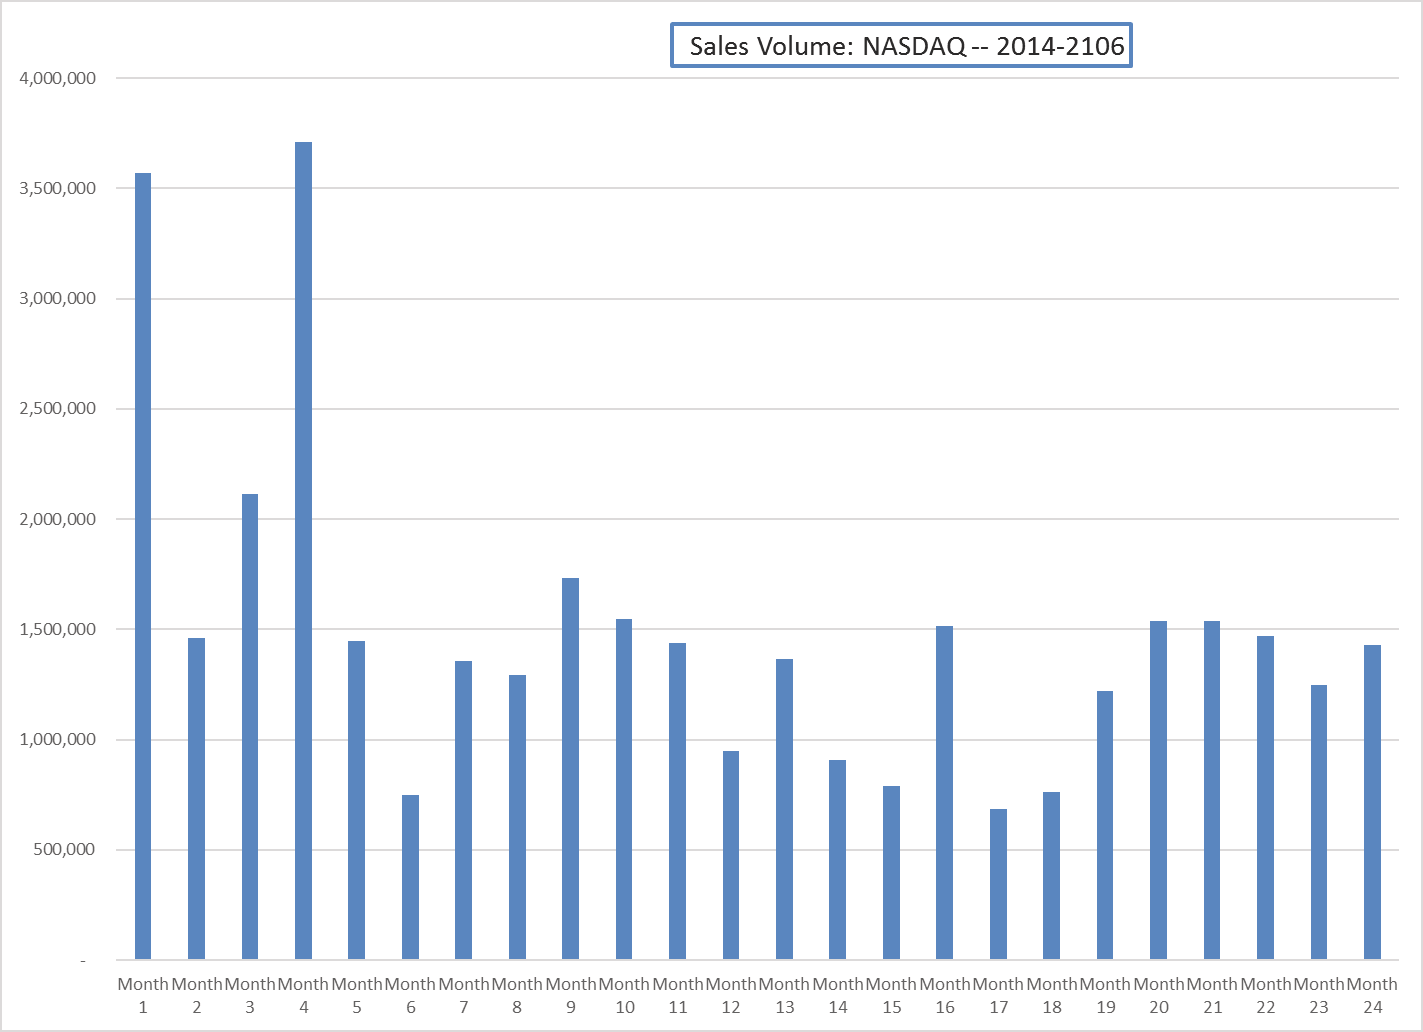
\includegraphics[width=\maxwidth{.95\linewidth}]{gfx/ch04_fig01}
	\caption{Stock Trends}
	\label{04:fig01}
\end{figure}

Before creating the line chart, it is important to identify why it is an appropriate chart type given the message being communicated and the data available. When presenting the trend for any data over a designated period of time, the most commonly used chart types are the line chart and the column chart. A column chart is limited to a certain number of bars or data points. As the number of bars increases it becomes increasingly difficult to read. The worksheet contains 24 points of data that were used to construct the chart shown in Figure \ref{04:fig01}. This is generally too many data points to put on a column chart, which is why a line chart is a better choice. The line chart will show the volume of sales for the NASDAQ on the Y axis and the Month number on the X axis. The following steps explain how to construct this chart.

\textit{Data file: CH4 Data}

\begin{enumerate}
	\item Open data file \textbf{CH4 Data} and save it as \textbf{CH4 Charting}.
	\item Navigate to the \textbf{Stock Trend} worksheet.
	\item Highlight the range \textsf{B4:C28} on the \textbf{Stock Trend} worksheet. (Note that a label in the first row and more labels in column B are selected. Watch where they show up in the completed chart.)
	\item Click the Insert tab of the ribbon.
	\item Click the \textbf{Line} button in the \textbf{Charts} group of commands. Click the first option from the list, which is a basic 2D Line Chart (see Figure \ref{04:fig02}).
\end{enumerate}

\begin{figure}[H]
	\centering
	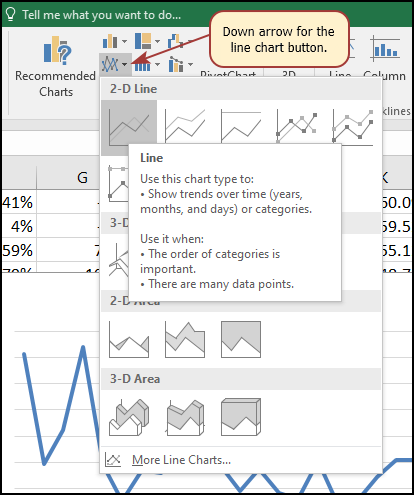
\includegraphics[width=\maxwidth{.95\linewidth}]{gfx/ch04_fig02}
	\caption{Selecting the Basic Line Chart}
	\label{04:fig02}
\end{figure}

This adds, or embeds, the line chart to the worksheet, as shown in Figure \ref{04:fig03}. Notice where the labels showed up on the chart.

\begin{center}
	\begin{infobox}{Why?}
		\textbf{Line Chart vs. Column Chart}
		\\
		\\
		Both a line chart and a column chart can be used to illustrate a trend over time. However, a line chart is far more effective when there are many periods of time being measured. For example, if fifty-two weeks are being reported a column chart would require fifty-two bars. A general rule of thumb is to use a column chart when twenty bars or fewer are required. A column chart becomes difficult to read as the number of bars exceeds twenty.
	\end{infobox}
\end{center}

Notice that additional tabs, or contextual tabs, are added to the ribbon when a chart is selected. We will demonstrate the commands in these tabs throughout this chapter. These tabs appear only when the chart is activated.

\begin{figure}[H]
	\centering
	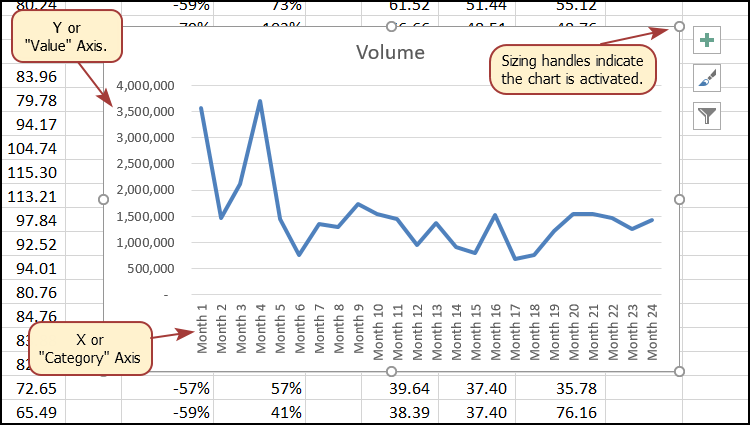
\includegraphics[width=\maxwidth{.95\linewidth}]{gfx/ch04_fig03}
	\caption{Embedded Line Chart in the Stock Trend Worksheet}
	\label{04:fig03}
\end{figure}

As shown in Figure \ref{04:fig03}, the embedded chart is not placed in an ideal location on the worksheet since it is covering several cell locations that contain data. The following steps demonstrate common adjustments that are made when working with embedded charts.

1. Moving a chart: Click and drag the upper left corner of the chart to the corner of cell B30.
2. Resizing a chart: Place the mouse pointer over the right upper corner sizing handle, hold down
the ALT key on your keyboard, and click and drag the chart so it “snaps” to the right side of
Column I.
3. Repeat step 2 to resize the chart so the top “snaps” to the top of Row 30, the bottom ``snaps'' to the bottom of Row 45, and the left side “snaps” to the left side of Column B. Make sure the right side of the chart snaps to the line between column I and J.
4.   Adjusting the chart title: Click the chart title once. Then click in front of the first letter. You
should see a blinking cursor in front of the letter. This allows you to modify the title of the chart.
5.   Type the following in front of the first letter in the chart title: May 2014-2016 Trend for NASDAQ Sales.
6.   Click anywhere outside of the chart to deactivate it.
7.   Save your work.

Note: Excel 2010 uses three contextual tabs for charts. Later versions use only two. Each has all the same tools. They are just organized a little differently.

Figure 4.4 shows the line chart after it is moved and resized. You can also see that the title of the chart has been edited to read May 2014-2016 Trend for NASDAQ Sales Volume. Notice that the sizing handles do not appear around the perimeter of the chart. This is because the chart has been deactivated. To activate the chart, click anywhere inside the chart perimeter.

\begin{tabular}{p{3.25in}p{0.5in}} %Max width: 4.25in
	\hline
	\textit{Note:} The pointer will change into the shape illustrated on the right when it is in the right place to \textbf{move} the chart. & \raisebox{-0.30in}{
\includegraphics[]{gfx/ch04_fig99}} \\
	\hline
	\textit{Note:} The pointer will change into the shape illustrated on the right when it is in the right place to \textbf{resize} the chart. & \raisebox{-0.30in}{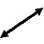
\includegraphics[]{gfx/ch04_fig98}} \\
	\hline
\end{tabular}


\begin{figure}[H]
	\centering
	
\includegraphics[width=\maxwidth{.95\linewidth}]{gfx/ch04_fig04}
	\caption{Line Chart Moved and Resized}
	\label{04:fig04}
\end{figure}

\begin{center}
	\begin{sklbox}{Skill Refresher}
		\textbf{Inserting a Line Chart}
		\\
		\begin{itemize}
			\setlength{\itemsep}{0pt}
			\setlength{\parskip}{0pt}
			\setlength{\parsep}{0pt}

			\item Highlight a range of cells that contain data that will be used to create the chart. Be sure to include labels in the selection.
			\item Click the Insert tab of the ribbon.
			\item Click the Line button in the Charts group.
			\item Select a format option from the Line Chart drop-down menu.
			
		\end{itemize}
	\end{sklbox}
\end{center}

\begin{center}
	\begin{infobox}{Integrity Check}
		\textbf{Category Axis}
		\\
		\\
		When using line charts in Excel, keep in mind that anything placed on the X axis is considered a descriptive label, not a numeric value. This is an example of a category axis. This is important because there will never be a change in the spacing of any items placed on the X axis of a line chart. If numeric data must be placed on the category axis the chart will need to be modified. That process is covered later in the chapter.		
	\end{infobox}
\end{center}




\subsubsection{Adjusting the Y Axis Scale}

After creating an Excel chart, you may find it necessary to adjust the scale of the Y axis. Excel
automatically sets the maximum value for the Y axis based on the data used to create the chart. The
minimum value is usually set to zero. That is usually a good thing. However, depending on the data
you are using to create the chart, setting the minimum value to zero can substantially minimize the
graphical presentation of a trend. For example, the trend shown in Figure 4.4 appears to be increasing
slightly in recent months. The presentation of this trend can be improved if the minimum value
started at 500,000. The following steps explain how to make this adjustment to the Y axis:

1. Click anywhere on the Y (value or vertical) axis on the May 2014-2016 Trend for NASDAQ
Sales Volume line chart (Stock Trend worksheet).
2. Right Click and select Format Axis. The Format Axis Pane should appear, as shown in Figure
4.5.




Note: If you do not see “Format Axis . . . on your menu, you have not right clicked in the correct spot.
Press “Escape” to turn the menu off and try again


\begin{figure}[H]
	\centering
	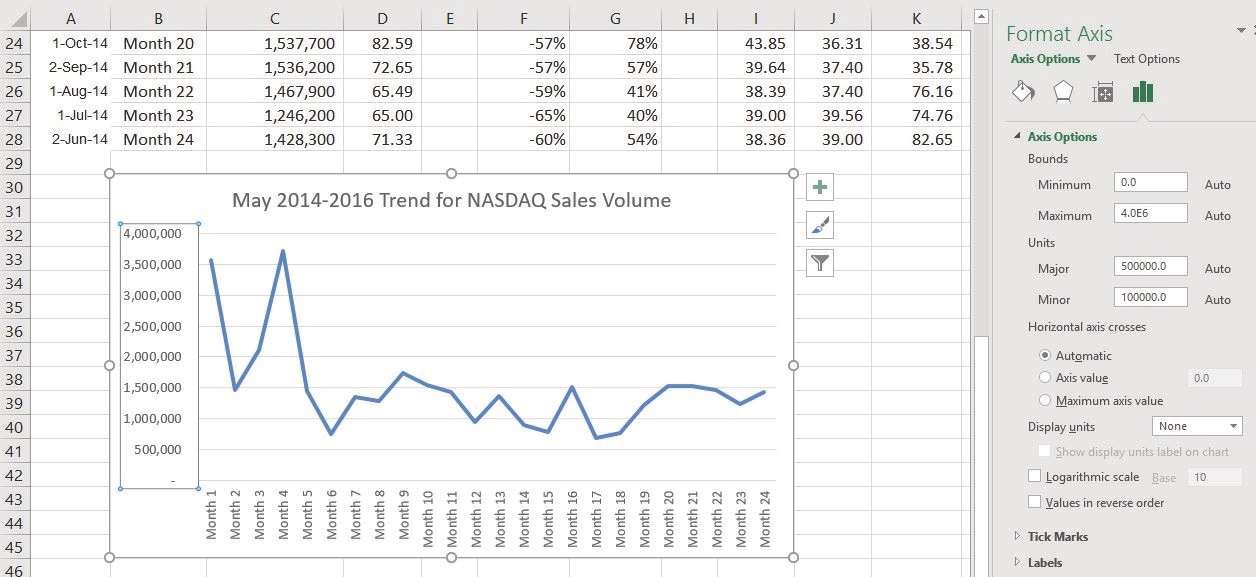
\includegraphics[width=\maxwidth{.95\linewidth}]{gfx/ch04_fig05}
	\caption{Format Axis Pane}
	\label{04:fig05}
\end{figure}






1. In the Format Axis Pane, click the input box for the “Minimum” axis option and delete the zero.
Then type the number 500000 and hit Enter. As soon as you make this change, the Y axis on the
chart adjusts.
2. Click the X in the upper right corner of the Format Axis pane to close it.
3. Save your work.

Figure 4.6 shows the change in the presentation of the trend line. Notice that with the Y axis starting
at 500,000, the trend for the NASDAQ is more pronounced. This adjustment makes it easier for the
audience to see the magnitude of the trend.



\begin{figure}[H]
	\centering
	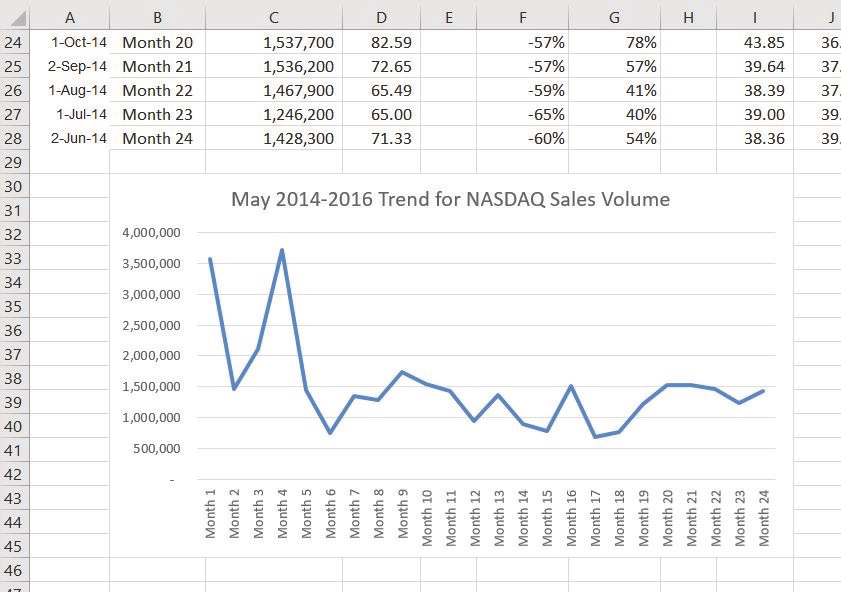
\includegraphics[width=\maxwidth{.95\linewidth}]{gfx/ch04_fig06}
	\caption{Adjusted Y Axis for the S\&P 500 Chart}
	\label{04:fig06}
\end{figure}




\begin{center}
	\begin{sklbox}{Skill Refresher}
		\textbf{Adjusting the Y Axis Scale}
		\\
		\begin{itemize}
			\setlength{\itemsep}{0pt}
			\setlength{\parskip}{0pt}
			\setlength{\parsep}{0pt}

			\item Click anywhere along the Y axis to activate it.
			\item Right Click. (\textit{Note}: you can also select the Format tab in the Chart Tools section of the ribbon.)
			\item Select Format Axis . . .
			\item In the Format Axis pane, make the changes to the Axis Options.
			\item Click in the input box next to the desired axis option and then type the new scale value.
			\item Click the Close button at the top right of the Format Axis pane to close it.
			
		\end{itemize}
	\end{sklbox}
\end{center}

\subsection{Trend Comparisons: Line Chart 2}

We will now create a second line chart using the data in the Stock Trend worksheet. The purpose of
this chart is to compare two trends: the change in volume for the NASDAQ and the change in the
Closing price.

Before creating the chart to compare the NASDAQ volume and sales price, it is important to review
the data in the range B4:D28 on the Stock Trend worksheet. We cannot use the volume of sales and the
closing price because the values are not comparable. That is, the closing price is in a range of $45.00
to $115.00, but the data for the volume of Sales is in a range of 684,000 to 3,711,000. If we used these
values – without making changes to the chart — we would not be able to see the closing price at all.


The construction of this second line chart will be similar to the first line chart. The X axis will be the
months in the range B4:D28.

1.   Highlight the range B4:D28 on the Stock Trend worksheet.
2.   Click the Insert tab of the ribbon.
3.   Click the Line button in the Charts group of commands.
4.   Click the first option from the list, which is a basic line chart.

Figure 4.6.5 shows the appearance of the line chart comparing both the volume and the closing price
before it is moved and resized. Notice that the line for the closing price (Close) appears as a straight
line at the bottom of the chart. Also, the chart is covering the data again, and the title needs to be
changed.


\begin{figure}[H]
	\centering
	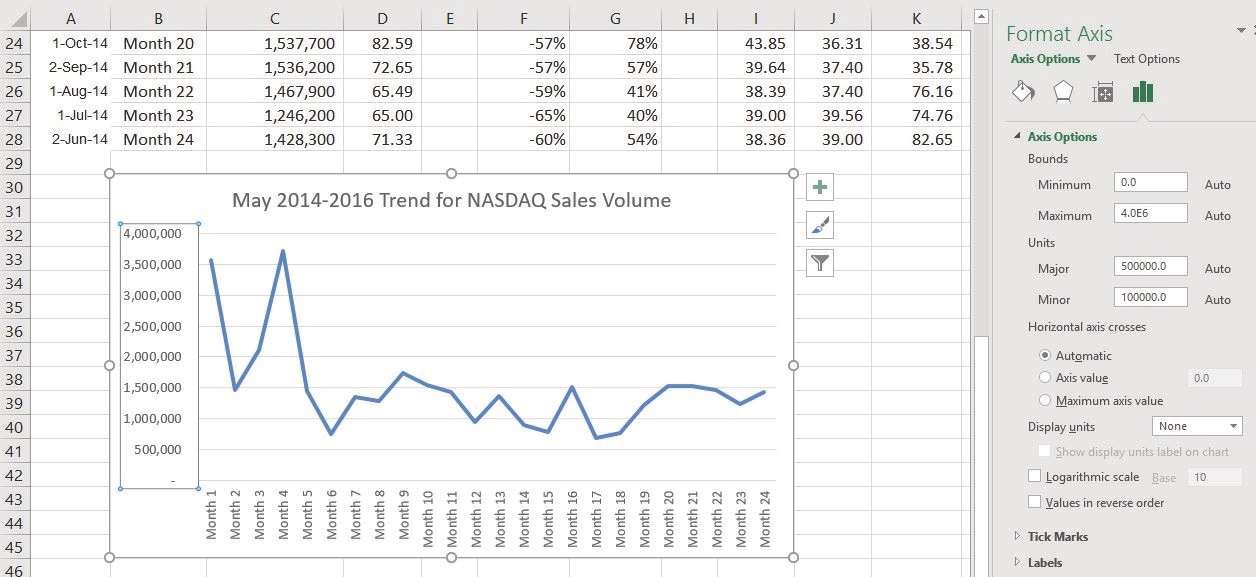
\includegraphics[width=\maxwidth{.95\linewidth}]{gfx/ch04_fig07}
	\caption{Trend Comparison Line Chart}
	\label{04:fig07}
\end{figure}





1. Move the chart so the upper left corner is in the middle of cell M3.
2. Resize the chart, using the resizing handles and the ALT key, so the left side is locked to the left




Note: The line representing the closing values is flat along the bottom of the chart. This is hard to see
and not very useful as is. Fear not. We will fix that.





side of Column M, the right side is locked to the right side of Column U, the top is locked to the
top of Row 3, and the bottom is locked to the bottom of Row 17.
3. Click in the text box that says “Chart Title.” Delete the text and replace it with the following: 24
Month Trend Comparison.

Good. But, we still cannot really see the Closing Price data. It is the flat red line at the very bottom of
the chart.

1. Right click the red line across the bottom of the chart that represents the Closing Price.
2. On the menu, select Format Data Series. This will open the Format Data Series pane.
3. In the Series Options, select Secondary Axis.


\begin{figure}[H]
	\centering
	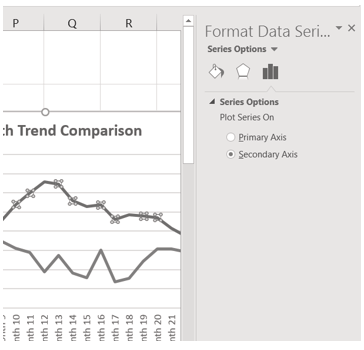
\includegraphics[width=\maxwidth{.95\linewidth}]{gfx/ch04_fig08}
	\caption{Adding a Secondary Axis}
	\label{04:fig08}
\end{figure}





Better! But, it would be nice to be able to see that the values on the right represent prices.

1.   Right click the Secondary Vertical Axis. (The vertical axis on the right that goes from 0 to 140.)
2.   From the menu, select Format Axis.
3.   In Axis Options, select Number. (You may have to scroll down to see it.)
4.   Use the Symbol list box to add the \$.
5.   Press the Close button to close the Format Axis pane.
6.   Save your work.



\begin{figure}[H]
	\centering
	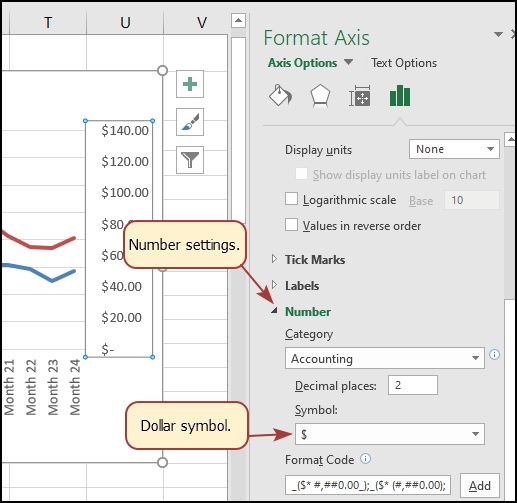
\includegraphics[width=\maxwidth{.95\linewidth}]{gfx/ch04_fig09}
	\caption{Modifying the Secondary Axis}
	\label{04:fig09}
\end{figure}





\begin{figure}[H]
	\centering
	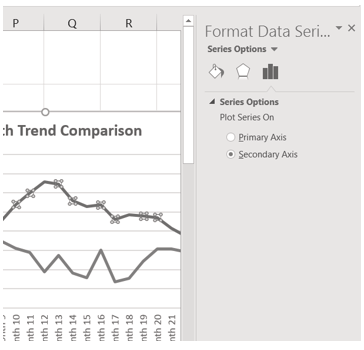
\includegraphics[width=\maxwidth{.95\linewidth}]{gfx/ch04_fig10}
	\caption{Final Comparison Line Chart}
	\label{04:fig10}
\end{figure}





\subsection{``Instant'' Chart – F11}

On the Stock Trend worksheet:

1. Select A4:A28.
2. Hold down the Ctrl key and select D4:D28. Figure 4.10 shows what that will look like.


\begin{figure}[H]
	\centering
	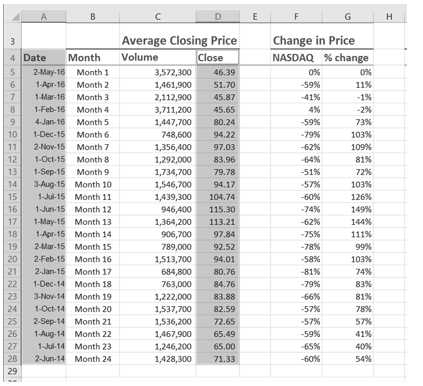
\includegraphics[width=\maxwidth{.95\linewidth}]{gfx/ch04_fig11}
	\caption{Range Selection}
	\label{04:fig11}
\end{figure}





3. Press F11. (The F11 function key is on the top row of the keyboard.) If the factory default
settings haven’t been changed, Excel will create a column chart and place it on a separate chart
sheet. (See Figure 4.11).
4. Change the name of the chart sheet by double-clicking the worksheet name Chart1. Type
Closing Prices as the new name and hit Enter.
5. Save your work.



\begin{figure}[H]
	\centering
	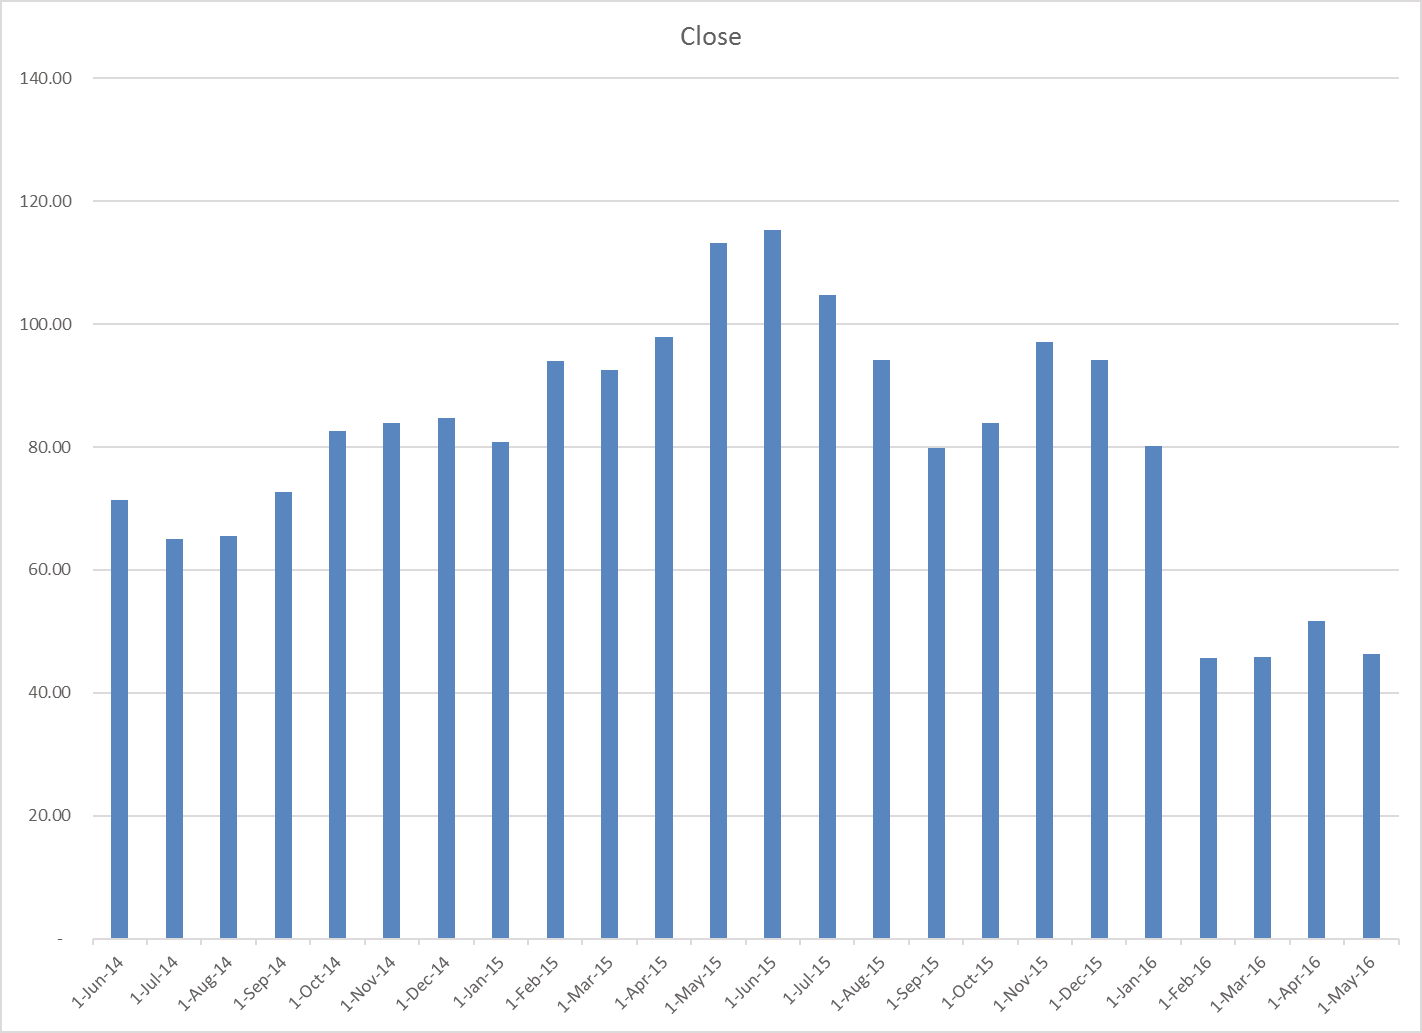
\includegraphics[width=\maxwidth{.95\linewidth}]{gfx/ch04_fig12}
	\caption{Instant Chart}
	\label{04:fig12}
\end{figure}





\subsection{Frequency Distribution: Column Chart 1}

A column chart is commonly used to show trends over time, as long as the data are limited to
approximately twenty points or less. A common use for column charts is frequency distributions. A
frequency distribution shows the number of occurrences by established categories. For example, a
common frequency distribution used in most academic institutions is a grade distribution. A grade
distribution shows the number of students that achieve each level of a typical grading scale (A, A-, B+,
B, etc.). The Grade Distribution worksheet contains final grades for some hypothetical Excel classes.
To show the grade frequency distribution for all the Excel classes in that year, the numbers of students
appear on the Y axis and the grade categories appear on the X axis. The number of students for this
chart is in Column C. The labels for grades are in Column A. The following steps explain how to
create this chart:

1. Select the Grade Distribution worksheet.
2. Change the years in Row3 to the current academic term and year.
3. Highlight the range A3:A8 on the Grade Distribution worksheet. Column A shows the grade
categories.
4. Hold down the Crtl key.
5. Without letting go of the Ctrl key, select C3:C8


6. Click the Column button in the Charts group section on the Insert tab of the ribbon. Select the
first option in the 2-D Column section, which is the Clustered Column format.
7. Click and drag the chart so the upper left corner is in the middle of cell H2.
8. Resize the chart so the left side is locked to the left side of Column H, the right side is locked to
the right side of Column O, the top is locked to the top of Row 2, and the bottom is locked to the
bottom of Row 16.
9. If Excel displays a legend, delete it by clicking the legend one time and pressing the DELETE key
on the keyboard. Since the chart presents only one data series, the legend is not necessary.
10. Add the text Final Grades for to the chart title. The chart title should now be Final Grades for
All Excel Classes 2016/2017 (or whichever academic year you are using).
11. Click any cell location on the Grade Distribution worksheet to deactivate the chart.
12. Save your work.

Figure 4.12 shows the completed grade frequency distribution chart. By looking at the chart, you can
immediately see that the greatest number of students earned a final grade in the B+ to B- range.


\begin{figure}[H]
	\centering
	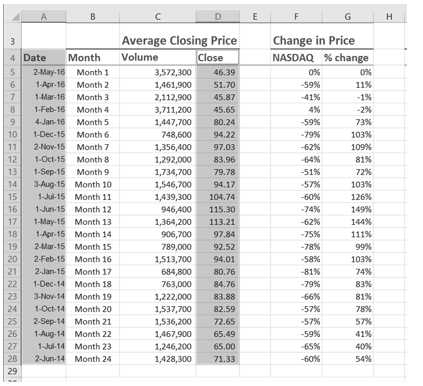
\includegraphics[width=\maxwidth{.95\linewidth}]{gfx/ch04_fig13}
	\caption{Grade Frequency Distribution Chart}
	\label{04:fig13}
\end{figure}

\subsection{Creating a Chart Sheet}

The charts we have created up to this point have been added to, or embedded in, an existing
worksheet (with the exception of the Instant Chart we created using F11). Charts can also be placed
in a dedicated worksheet called a chart sheet. It is called a chart sheet because it can only contain an
Excel chart. Chart sheets are useful if you need to create several charts using the data in a single
worksheet. If you embed several charts in one worksheet, it can be cumbersome to navigate and
browse through the charts. It is easier to browse through charts when they are moved to a chart
sheet because a separate sheet tab is added to the workbook for each chart. The following steps
explain how to move the grade frequency distribution chart to a dedicated chart sheet:




1. Click anywhere on the Final Grades for All Excel Classes chart on the Grade Distribution
worksheet.
2. Right click on the chart. Select Move Chart . . . This opens the Move Chart Dialog box.
3. Click the New sheet option on the Move Chart dialog box. (The top option.)
4. The entry in the input box for assigning a name to the chart sheet tab should automatically be
highlighted once you click the New sheet option. Type All Excel Classes. This replaces the
generic name in the input box (see Figure 4.13).
5. Click the OK button at the bottom of the Move Chart dialog box. This adds a new chart sheet to
the workbook with the name All Excel Classes.
6. Save your work.




Why?

Column Chart vs. Bar Chart

When using charts to show frequency distributions, the difference between a column chart and a bar chart is
really a matter of preference. Both are very effective in showing frequency distributions. However, if you are
showing a trend over a period of time, a column chart is preferred over a bar chart. This is because a period of
time is typically shown horizontally, with the oldest date on the far left and the newest date on the far right.
Therefore, the descriptive categories for the chart would have to fall on the horizontal – or category axis, which is
the configuration of a column chart. On a bar chart, the descriptive categories are displayed on the vertical axis.


\begin{figure}[H]
	\centering
	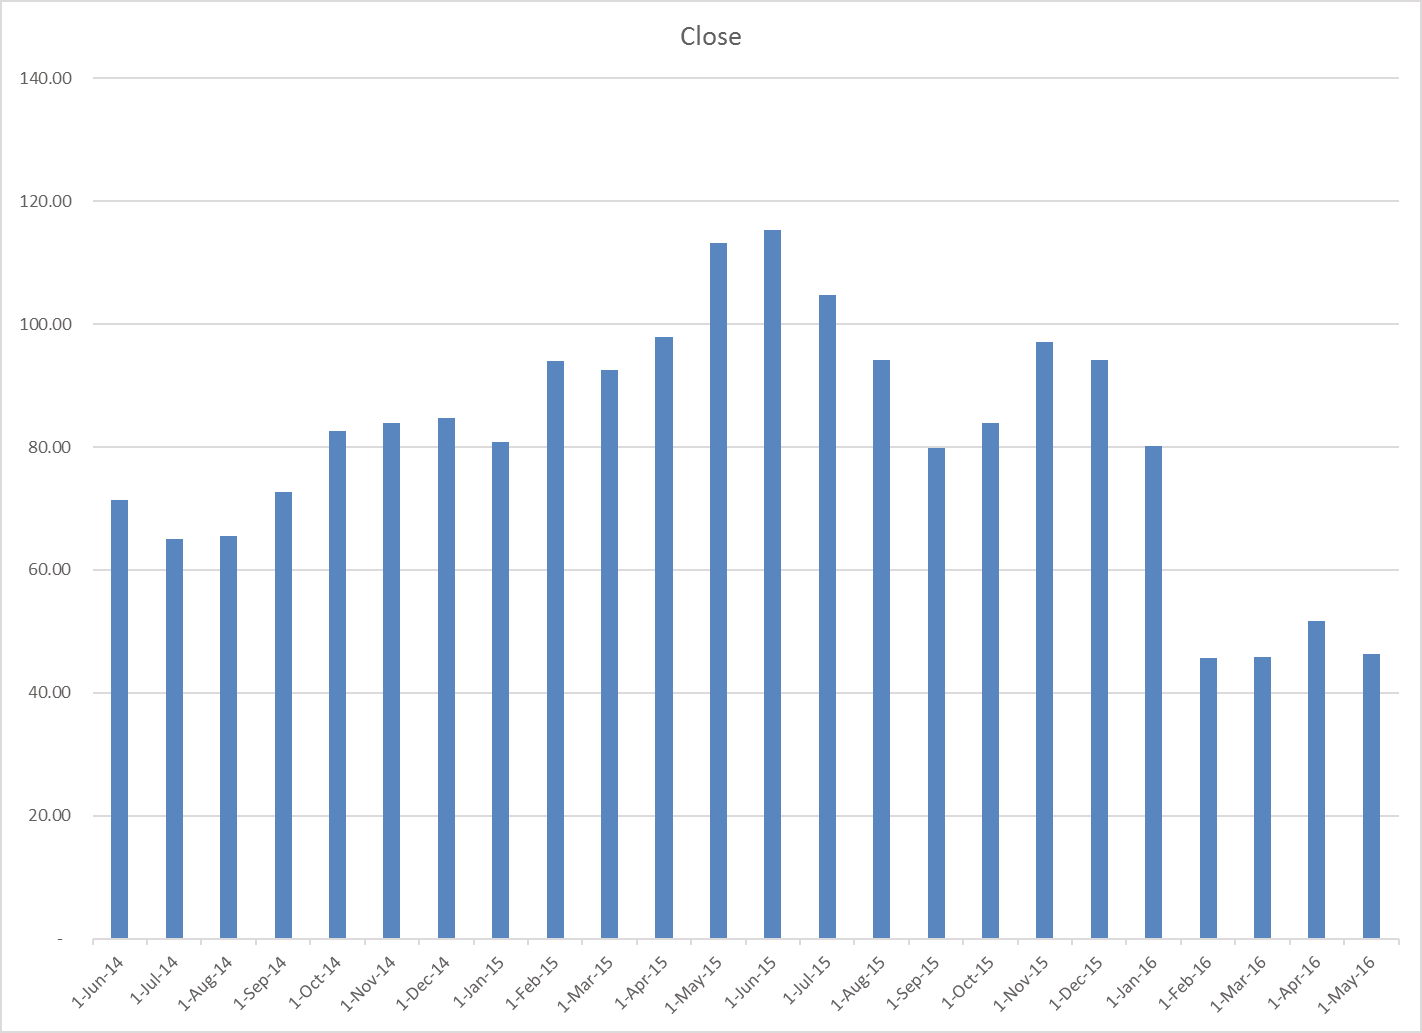
\includegraphics[width=\maxwidth{.95\linewidth}]{gfx/ch04_fig14}
	\caption{Moving a Chart to a Chart Sheet}
	\label{04:fig14}
\end{figure}



Figure 4.14 shows the Final Grades for the all the Excel Classes column chart is in a separate chart
sheet. Notice the new worksheet tab added to the workbook matches the New sheet name entered
into the Move Chart dialog box. Since the chart is moved to a separate chart sheet, it no longer is
displayed in the Grade Distribution worksheet.


\begin{figure}[H]
	\centering
	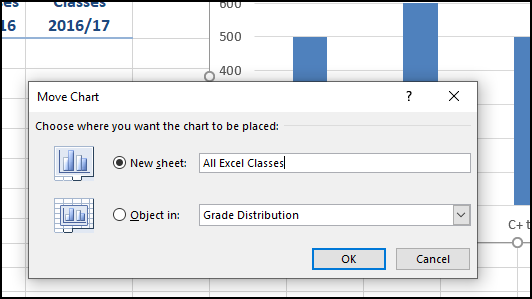
\includegraphics[width=\maxwidth{.95\linewidth}]{gfx/ch04_fig15}
	\caption{Chart Sheet Added to the Workbook}
	\label{04:fig15}
\end{figure}






\subsection{Frequency Comparison: Column Chart 2}

We will create a second column chart to show a comparison between two frequency distributions.
Column B on the Grade Distribution worksheet contains data showing the number of students who
received grades within each category for the Spring Quarter. We will use a column chart to compare
the grade distribution for Spring (Column B) with the overall grade distribution for the whole year
(Column C).

However, since the number of students in the term is significantly different from the total number
of students in the year, we must calculate percentages in order to make an effective comparison. The
following steps explain how to calculate the percentages:

1. Highlight the range B9:C9 on the Grade Distribution worksheet.
2. Click the AutoSum button in the Editing group of commands on the Home tab of the ribbon.
This automatically adds SUM functions that sum the values in the range B4:B8 and C4:C8.
3. Activate cell E4 on the Grade Distribution worksheet.
4. Enter a formula that divides the value in cell B4 by the total in cell B9. Add an absolute reference
to cell B9 in the formula =B4/$B$9.
5. Copy the formula in cell E4 and paste it into the range E5:E8 using the Paste command.
Or, use the Fill Handle to copy the calculation in E4 all the way down to E8.
6. Activate cell F4 on the Grade Distribution worksheet.


7. Enter a formula that divides the value in cell C4 by the total in cell C9. Add an absolute reference
to cell C9 in the formula =C4/$C$9.
8. Copy the formula in cell F4 and paste it into the range F5:F8 using the Paste command.
Or, use the Fill Handle to copy the calculation in F4 all the way down to F8.



\begin{figure}[H]
	\centering
	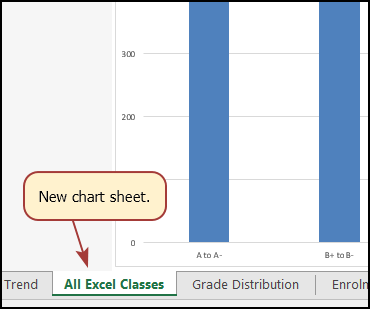
\includegraphics[width=\maxwidth{.95\linewidth}]{gfx/ch04_fig16}
	\caption{Completed Grade Distribution Percentages}
	\label{04:fig16}
\end{figure}




Figure 4.15 shows the completed percentages added to the Grade Distribution worksheet.

The column chart we are going to create uses the grade categories in the range A4:A8 on the X axis
and the percentages in the range E4:F8 on the Y axis. This chart uses data that is not in a contiguous
range, so we need to use the Ctrl key to select the ranges of cells.

1. Select A3:A8, hold down the Ctrl key and select E3:F8.
2. Click the Insert tab of the ribbon.
3. Click the Column button in the Charts group of commands. Select the first option from the
drop-down list of chart formats, which is the Clustered Column.
4. Click and drag the chart so the upper left corner is in the middle of cell H2.
5. Resize the chart so the left side is locked to the left side of Column H, the right side is locked to
the right side of Column N, the top is locked to the top of Row 2, and the bottom is locked to the
bottom of Row 16.
6. Change the chart title to Grade Distribution Comparison. If you do not have a chart title, you



can add one. On the Design tab, select Add Chart Element. Find the Chart Title. Select the
Above Chart option from the drop-down list.
7. Save your work.


\begin{figure}[H]
	\centering
	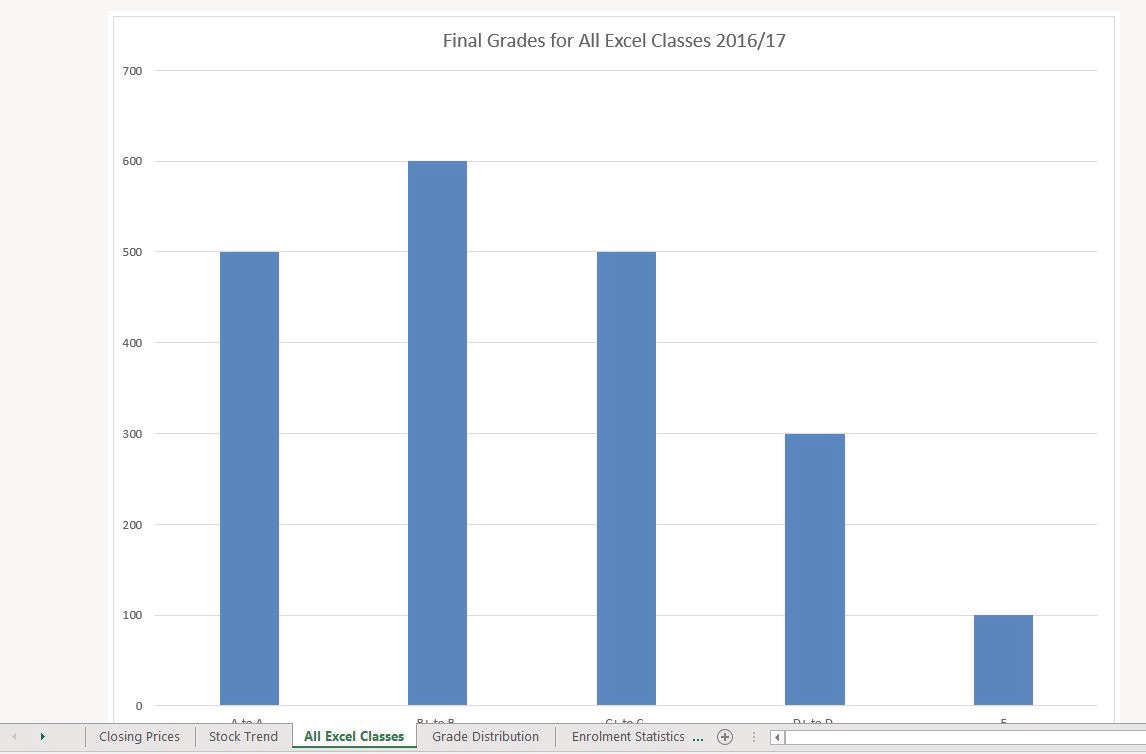
\includegraphics[width=\maxwidth{.95\linewidth}]{gfx/ch04_fig17}
	\caption{Completed Data Series for the Class Grade Distribution}
	\label{04:fig17}
\end{figure}





Figure 4.17 shows the final appearance of the column chart. The column chart is an appropriate type
for this data because there are fewer than twenty data points and we can easily see the comparison
for each category. An audience can quickly see that the class issued fewer As compared to the college.
However, the class had more Bs and Cs compared with the college population.


\begin{figure}[H]
	\centering
	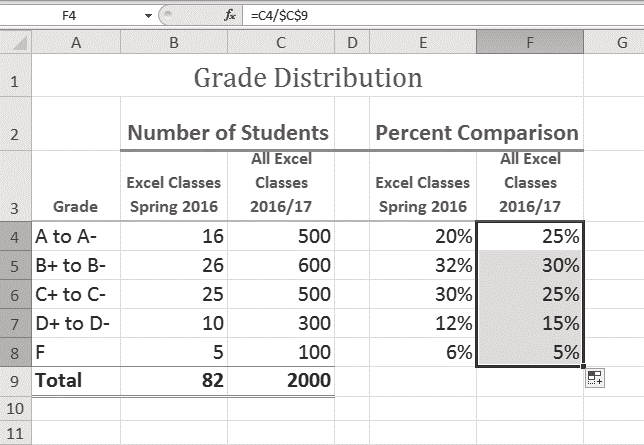
\includegraphics[width=\maxwidth{.95\linewidth}]{gfx/ch04_fig18}
	\caption{Completed Grade Distribution Column Chart}
	\label{04:fig18}
\end{figure}

\begin{center}
	\begin{infobox}{Integrity Check}
		\textbf{Too Many Bars on a Column Chart?}
		\\
		\\
		 Although there is no specific limit for the number of bars you should use on a column chart, a general rule of thumb is twenty bars or less. Figure \ref{04:fig21} contains a total of thirty-two bars. This is considered a poor use of a column chart because it is difficult to identify meaningful trends or comparisons. The data used to create this chart might be better used in two or three different column charts, each with a distinct idea or message.
	\end{infobox}
\end{center}

\begin{figure}[H]
	\centering
	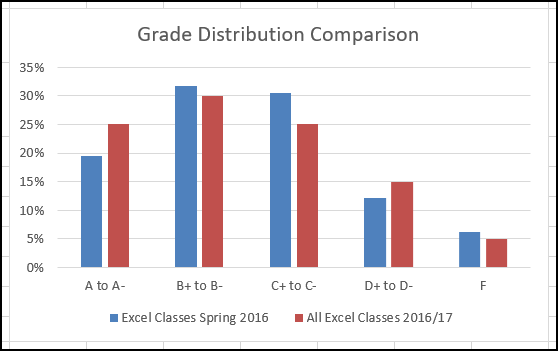
\includegraphics[width=\maxwidth{.95\linewidth}]{gfx/ch04_fig19}
	\caption{Poor Use of a Column Chart}
	\label{04:fig19}
\end{figure}

\subsection{Percent of Total: Pie Chart}

The next chart we will demonstrate is a pie chart. A pie chart is used to show a percent of total for
a data set at a specific point in time. The data we will use to demonstrate a pie chart is related to
enrollment data for Portland Area Community Colleges for Fall of 2014. You will find that data on
the Enrollment Statistics sheet.

1.   Highlight the range A2:B6 on the Enrollment Statistics worksheet.
2.   Click the Insert tab of the ribbon.
3.   Click the Pie button in the Charts group of commands.
4.   Select the first “2-D Pie” option from the drop-down list of options.
5.   To make the “slices” stand out better, “explode” the pie chart.

* Click and hold the mouse button down in any of the slices of the pie.
* Note that you have selection handles on all of the pie slices.
* Without letting go of your mouse button; drag one of the slices away from the center.
* All of the slices “explode” out from the center.



1. Click off the slices and into the white canvas to deselect the pie and select the entire chart.
2. Click and drag the pie chart so the upper left corner is in the middle of cell E2.
3. Resize the pie chart so the left side is locked to the left side of Column E, the right side is locked
to the right side of Column L, the top is locked to the top of Row 2, and the bottom is locked to
the bottom of Row 10 (see Figure 4.19).



\begin{figure}[H]
	\centering
	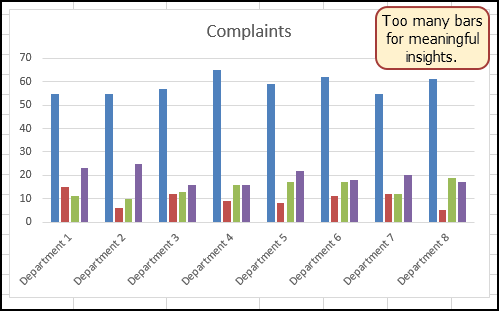
\includegraphics[width=\maxwidth{.95\linewidth}]{gfx/ch04_fig20}
	\caption{Pie Chart Moved and Resized}
	\label{04:fig20}
\end{figure}




1. Click the chart legend once and press the DELETE key on your keyboard. A pie chart typically
shows labels next to each slice. Therefore, the legend is not needed.
2. Right click any of the slices in the pie chart, and select Add Data Labels from the list. This will
add the values for each of the slices in the pie.
3. Now, you can right click one of the numbers and select Format Data Labels from the list. This
will open the Format Data Labels pane on the right.
4. Check the boxes for Category Name and Percentage in the Label Options section in the




Note: if you let go of the mouse button before dragging, you may only get one slice to move when you
drag it out from the center. This can be another option for displaying your data. Use the Undo button to
undo this if you want to try again.





Format Data Labels pane. This will add the Race/ethnicity labels as well as the percentage data
to the pie chart.
5.   Uncheck the box next to the Value box. This will remove the numbers from the pie chart (see
Figure 4.20).
6.   Click the Close button at the top of the Format Data Labels pane.
7.   Select the data labels again (if needed). Click the Home tab of the ribbon and then click the Bold
button. This will bold the data labels on the pie chart.
8.   Save your work.


\begin{figure}[H]
	\centering
	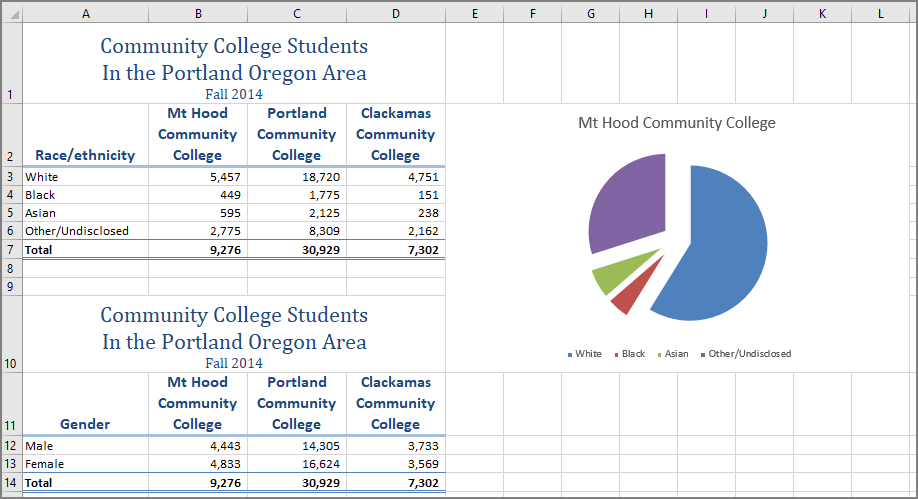
\includegraphics[width=\maxwidth{.95\linewidth}]{gfx/ch04_fig21}
	\caption{Final Settings in the Format Data Labels Pane}
	\label{04:fig21}
\end{figure}





Although there are no specific limits for the number of categories you can use on a pie chart, a good
rule of thumb is ten or less. As the number of categories exceeds ten, it becomes more difficult to
identify key categories that make up the majority of the total.



\begin{figure}[H]
	\centering
	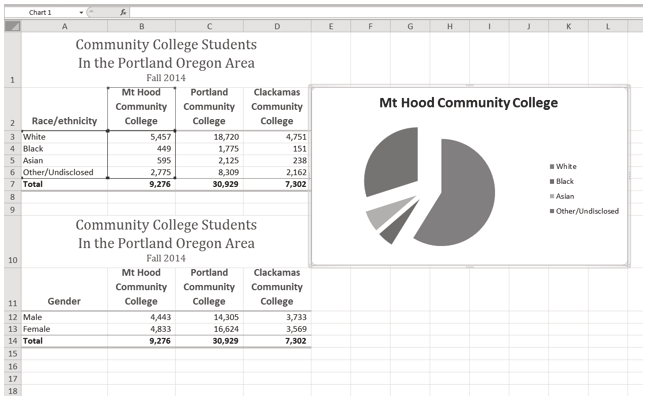
\includegraphics[width=\maxwidth{.95\linewidth}]{gfx/ch04_fig22}
	\caption{Final Enrollment Statistics Pie Chart}
	\label{04:fig22}
\end{figure}





\begin{center}
	\begin{sklbox}{Skill Refresher}
		\textbf{Inserting a Pie Chart}
		\\
		\begin{itemize}
			\setlength{\itemsep}{0pt}
			\setlength{\parskip}{0pt}
			\setlength{\parsep}{0pt}

			\item Highlight a range of cells that contain the data used to create the chart.
			\item Click the Insert tab of the ribbon.
			\item Click the Pie button in the Charts group.
			\item Select a format option from the Pie Chart drop-down menu.
			
		\end{itemize}
	\end{sklbox}
\end{center}


\subsection{Percent of Total: Stacked Column Chart}

The last chart type we will demonstrate is the stacked column chart. We use a stacked column chart to
show a percent of a total . For example, the data on the Enrollment Statistics worksheet shows student
enrollment by race for several colleges. We would like to see all of the data on all of the colleges.

1. Highlight the range A2:D6 on the Enrollment Statistics worksheet.
2. Click the Insert tab of the ribbon.
3. Click the Column button in the Charts group of commands. Select the 100\% Stacked Column
format option from 2-D Column section in the drop-down list (see Figure 4.22).



\begin{figure}[H]
	\centering
	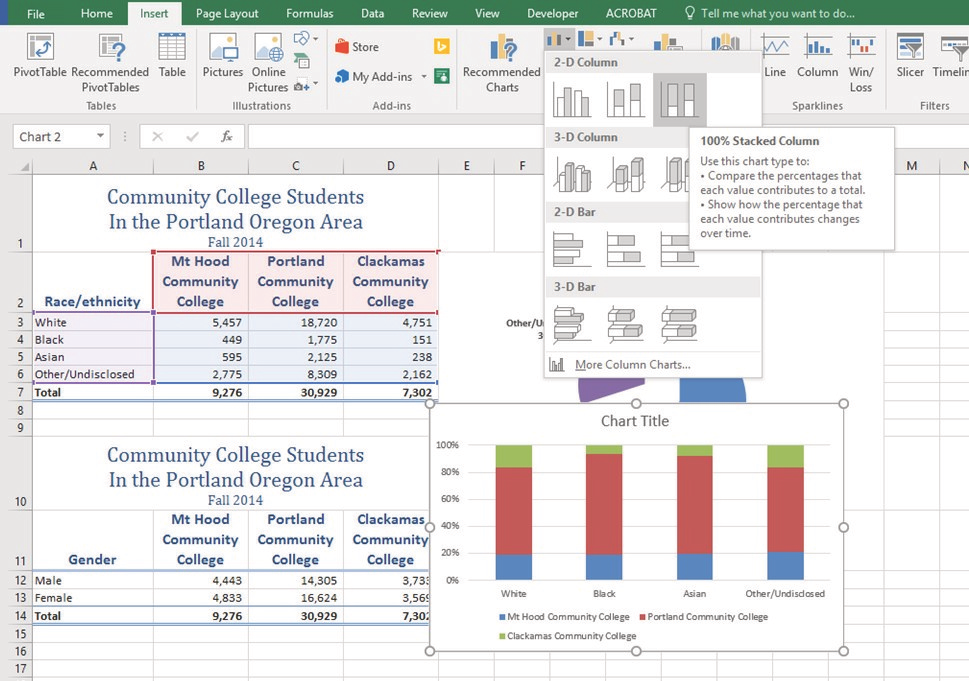
\includegraphics[width=\maxwidth{.95\linewidth}]{gfx/ch04_fig23}
	\caption{Selecting the 100\% Stacked Column Chart}
	\label{04:fig23}
\end{figure}


Figure 4.23 shows the column chart that is created after selecting the 100% Stacked Column format
option. As mentioned, the goal of this chart is to show the enrollment of students by race. However,
notice that Excel places the racial categories on the X axis. It would be more useful if the different
colleges were there instead.



\begin{figure}[H]
	\centering
	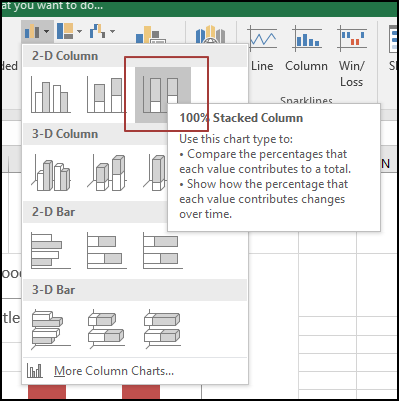
\includegraphics[width=\maxwidth{.95\linewidth}]{gfx/ch04_fig24}
	\caption{Initial Construction of the 100\% Stacked Column Chart}
	\label{04:fig24}
\end{figure}





The reason that Excel organized the data this way is that there are more Race/ethnicity categories
(data in column A) than there are colleges (data in row 2). Not a bad guess. But, not what we wanted
in this case.

The remaining steps explain how to correct this problem and complete the chart:

1. Click the Switch Row/Column button in the Design tab on the Chart Tools section of the
ribbon. This reverses the legend and current X axis categories.


\begin{figure}[H]
	\centering
	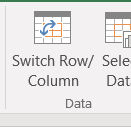
\includegraphics[width=\maxwidth{.95\linewidth}]{gfx/ch04_fig25}
	\caption{Switch Row/Column}
	\label{04:fig25}
\end{figure}





2. Click and drag the chart so the upper left corner is in the middle of cell E12.
3. Resize the chart so the left side is locked to the left side of Column E, the right side is locked to



the right side of Column N, the top is locked to the top of Row 12, and the bottom is locked to
the bottom of Row 30.
4. Click the legend one time and press the DELETE key on your keyboard.
5. Add a Data Table. This is another way of displaying a legend for a column chart along with the
numerical values that make up each component.

* In earlier versions of Excel, find the Labels group of commands and select the Show Data
Table with Legend Keys option from the drop-down menu.
* In Excel 2016, find the Add Chart Element tool on the Design tab, select Data Table With
Legend Keys

6. Change the Chart Title to Enrollment by Race.

* If there is no chart title, you will need to add one using the Add Chart Element tool on
the Design tab.

7. Save your work.

Figure 4.25 shows the final stacked column chart. Notice the similarities and differences in the
enrollment at the local community colleges.


\begin{figure}[H]
	\centering
	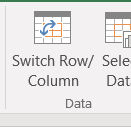
\includegraphics[width=\maxwidth{.95\linewidth}]{gfx/ch04_fig26}
	\caption{Final 100\% Stacked Column Chart}
	\label{04:fig26}
\end{figure}

\begin{center}
	\begin{sklbox}{Skill Refresher}
		\textbf{Inserting a Stacked Column Chart}
		\\
		\begin{itemize}
			\setlength{\itemsep}{0pt}
			\setlength{\parskip}{0pt}
			\setlength{\parsep}{0pt}

			\item Highlight a range of cells that contain data that will be used to create the chart.
			\item Click the Insert tab of the ribbon.
			\item Click the Column button in the Charts group.
			\item Select the Stacked Column format option from the Column Chart drop-down menu to show the values of each category on the Y axis. Select the 100\% Stacked Column option to show the percent of total for each category on the Y axis.
			
		\end{itemize}
	\end{sklbox}
\end{center}

\begin{center}
	\begin{tkwbox}{Key Take-Aways}
		\textbf{Save}
		\\
		\begin{itemize}
			\setlength{\itemsep}{0pt}
			\setlength{\parskip}{0pt}
			\setlength{\parsep}{0pt}
			
			\item Identifying the message you wish to convey to an audience is a critical first step in creating an Excel chart.
			\item Both a column chart and a line chart can be used to present a trend over a period of time. However, a line chart is preferred over a column chart when presenting data over long periods of time.
			\item The number of bars on a column chart should be limited to approximately twenty bars or less.
			\item When creating a chart to compare trends, the values for each data series must be within a reasonable range. If there is a wide variance between the values in the two data series (two times or more), the percent change should be calculated with respect to the first data point for each series.
			\item When working with frequency distributions, the use of a column chart or a bar chart is a matter of preference. However, a column chart is preferred when working with a trend over a period of time.
			\item A pie chart is used to present the percent of total for a data set.
			\item A stacked column chart is used to show how a percent total changes over time.

		\end{itemize}
	\end{tkwbox}
\end{center}


\section{Formatting Charts}


\begin{center}
	\begin{objbox}{Learning Objectives}
		\begin{itemize}
			\setlength{\itemsep}{0pt}
			\setlength{\parskip}{0pt}
			\setlength{\parsep}{0pt}

			\item Apply formatting commands to the X and Y axes.
			\item Enhance the visual appearance of the chart title and chart legend by using various formatting techniques.
			\item Assign titles to the X and Y axes that clarify labels and numeric values for the reader.
			\item Apply labels and formatting techniques to the data series in the plot area of a chart.
			\item Apply formatting commands to the chart area and the plot area of a chart.
			\item Employ series lines and annotations to enhance trends and provide additional information on a chart.
			
		\end{itemize}
	\end{objbox}
\end{center}


You can use a variety of formatting techniques to enhance the appearance of a chart once you have
created it. Formatting commands are applied to a chart for the same reason they are applied to a
worksheet: they make the chart easier to read. However, formatting techniques also help you qualify
and explain the data in a chart. For example, you can add footnotes explaining the data source as
well as notes that clarify the type of numbers being presented (i.e., if the numbers in a chart are
truncated, you can state whether they are in thousands, millions, etc.). These notes are also helpful
in answering questions if you are using charts in a live presentation. We will demonstrate these
formatting techniques using the column chart and stacked column chart from the previous section.

\subsection{X and Y Axis Formats}

There are numerous formatting commands we can apply to the X and Y axes of a chart. Although
adjusting the font size, style, and color are common, many more options are available through the
Format Axis pane. The following steps demonstrate a few of these formatting techniques on the
Grade Distribution Comparison chart:

1. Switch to the Grade Distribution worksheet and click anywhere along the X axis (horizontal
axis) of the Grade Distribution Comparison chart.
2. Right click and select Font.
3. Change the font to Arial, the Font Style to Bold, and the Size to 11 (see Figure 4.26).



\begin{figure}[H]
	\centering
	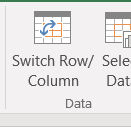
\includegraphics[width=\maxwidth{.95\linewidth}]{gfx/ch04_fig27}
	\caption{Font Dialog Box}
	\label{04:fig27}
\end{figure}





4. Click anywhere along the Y axis to activate it and repeat steps 2 and 3.
5. Click on the chart title and repeat steps 2 and 3, but set the Size to 14.
6. The final appearance of the axes is shown in Figure 4.27 Formatted X \& Y Axes.



\begin{figure}[H]
	\centering
	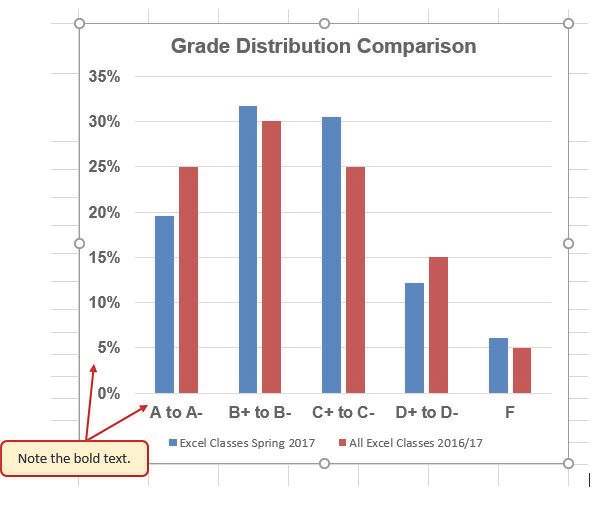
\includegraphics[width=\maxwidth{.95\linewidth}]{gfx/ch04_fig28}
	\caption{Formatted X and Y Axes}
	\label{04:fig28}
\end{figure}





Next we want to make some changes to the percentage numbers on the Y (vertical) axis.

1. Right click the vertical (value) axis. Select Format Axis. This opens the Format Axis pane.
2. Click Number from the list of options. The commands in this section of the Format Axis pane
are used to format numbers that appear on the selected axis of the chart.
3. Click in the Decimal places input box and change the value to 1.
4. Select Axis Options. Change the Minimum Bound to .05 to make the differences in the
columns more dramatic. The Format Axis pane should match Figure 4.28.
5. Click the Close button at the top of the Format Axis pane.
6. Save your work.


\begin{figure}[H]
	\centering
	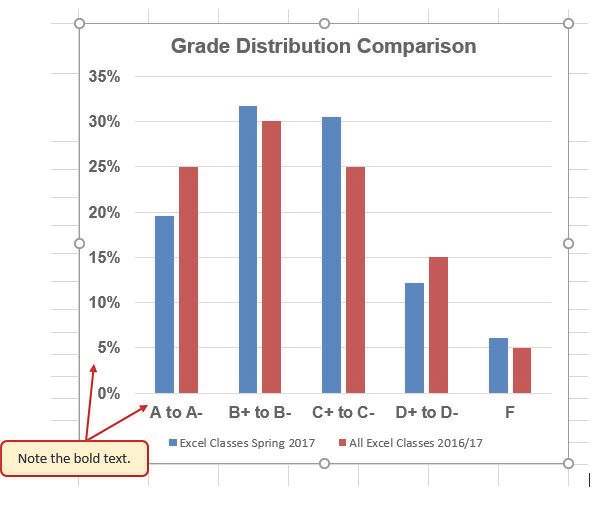
\includegraphics[width=\maxwidth{.95\linewidth}]{gfx/ch04_fig29}
	\caption{Format Axis Pane Changes}
	\label{04:fig29}
\end{figure}

Note: Experiment! You can also change font styling using shortcut keys and the buttons on the Home
tab.

\begin{center}
	\begin{sklbox}{Skill Refresher}
		\textbf{Formatting the X and Y Axes}
		\\
		\begin{itemize}
			\setlength{\itemsep}{0pt}
			\setlength{\parskip}{0pt}
			\setlength{\parsep}{0pt}

			\item Click anywhere along the X or Y axis to activate it.
			\item Click either the Home tab or Design tab of the ribbon.
			\item Select any of the available formatting commands in these tabs.
			
		\end{itemize}
	\end{sklbox}
\end{center}


\begin{center}
	\begin{sklbox}{Skill Refresher}
		\textbf{X and Y Axis Number Formats}
		\\
		\begin{itemize}
			\setlength{\itemsep}{0pt}
			\setlength{\parskip}{0pt}
			\setlength{\parsep}{0pt}

			\item Click anywhere along the X or Y axis to activate it.
			\item Click the Layout tab in the Chart Tools section of the ribbon.
			\item Click the Format Selection button in the Current Selection group of commands.
			\item Click Number from the list of options on the left side of the Format Axis dialog box.
			\item Select a number format and set decimal places on the right side of the Format Axis dialog box.
			\item Click the Close button in the Format Axis pane.
			
		\end{itemize}
	\end{sklbox}
\end{center}


\subsection{Chart Legend and Title Formats}

The next items we will format on the Grade Distribution Comparison chart are the chart legend and
title. Similar to the how we formatted the X and Y axes, we can format these items by activating them
and using the formatting commands in the Home tab or the Format pane. The following steps explain
how to add these formats:

1. Right click the legend on the Grade Distribution Comparison chart and select Format Legend.
2. Select Right in the Legend Position options. Close the Format Legend pane.
3. Move the legend by placing your cursor – shaped like a little plus sign with four arrows – on the
edge of the selection box. Click and drag the legend so the top of the legend aligns with the 35%
line next to the plot area (see Figure 4.29).



\begin{figure}[H]
	\centering
	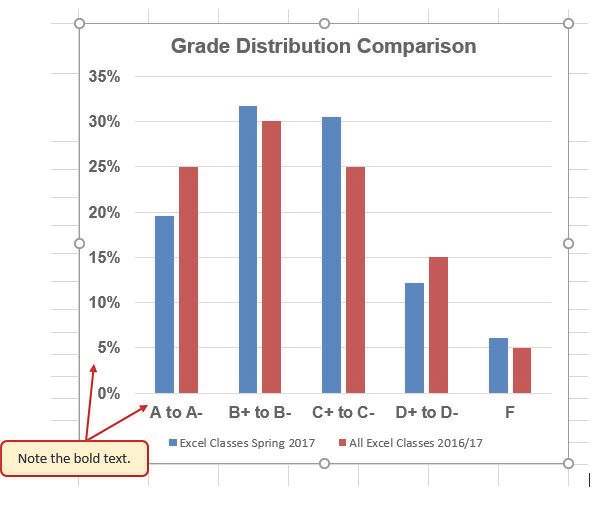
\includegraphics[width=\maxwidth{.95\linewidth}]{gfx/ch04_fig30}
	\caption{Moving the Legend}
	\label{04:fig30}
\end{figure}





1.   While the legend is still selected, change the font style in the Home tab of the ribbon to Arial.
2.   Change the font size to 12 points.
3.   Click the bold and italics commands in the Home tab of the ribbon.
4.   Click and drag the left sizing handle so the legend is against the plot area (see Figure 4.30).



\begin{figure}[H]
	\centering
	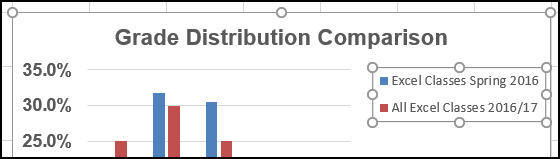
\includegraphics[width=\maxwidth{.95\linewidth}]{gfx/ch04_fig31}
	\caption{Legend Formatted and Resized}
	\label{04:fig31}
\end{figure}





1. Click the chart title to activate it.
2. Right click on the chart title and select Format Chart Title to open the Format Chart Title
pane.
3. Under Title Options , in the Effects group (the option in the middle) give your title one of the
Preset shadows. Change the color, if you like.
4. Close the Format Chart Title pane.
5. Save your work.



\begin{figure}[H]
	\centering
	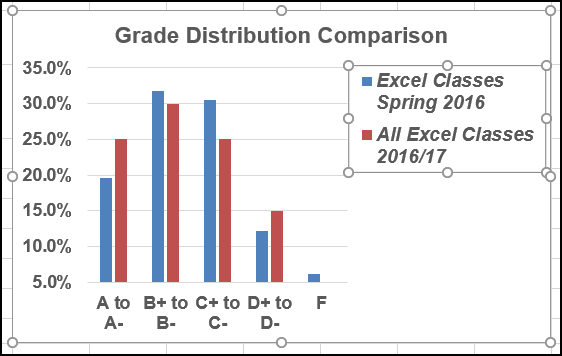
\includegraphics[width=\maxwidth{.95\linewidth}]{gfx/ch04_fig32}
	\caption{Format Chart Title Pane}
	\label{04:fig32}
\end{figure}

\begin{center}
	\begin{sklbox}{Skill Refresher}
		\textbf{Formatting the Chart Legend}
		\\
		\begin{itemize}
			\setlength{\itemsep}{0pt}
			\setlength{\parskip}{0pt}
			\setlength{\parsep}{0pt}

			\item Click the Legend to activate it.
			\item Click either the Home tab or right click to activate the appropriate formatting pane.
			\item Select any of the available formatting commands.
			\item Click and drag the legend to move it.
			\item Click and drag any of the sizing handles to adjust the size of the legend.
			
		\end{itemize}
	\end{sklbox}
\end{center}

\begin{center}
	\begin{sklbox}{Skill Refresher}
		\textbf{Formatting the Chart Title}
		\\
		\begin{itemize}
			\setlength{\itemsep}{0pt}
			\setlength{\parskip}{0pt}
			\setlength{\parsep}{0pt}

			\item Click anywhere on the chart title.
			\item Click either the Home tab or right click to activate the appropriate formatting pane.
			\item Select any of the available formatting commands.
			
		\end{itemize}
	\end{sklbox}
\end{center}

\subsection{X and Y Axis Titles}

Titles for the X and Y axes are necessary for defining the numbers and categories presented on a
chart. For example, by looking at the Grade Distribution Comparison chart, it is not clear what the
percentages along the Y axis represent. The following steps explain how to add titles to the X and Y
axes to define these numbers and categories:

1. Click anywhere on the Grade Distribution Comparison chart in the Grade Distribution
worksheet to activate it.
2. On the Design tab on the ribbon select the Add Chart Element button, then Axis Titles, then
Primary Vertical. (See Figure 4.32)


\begin{figure}[H]
	\centering
	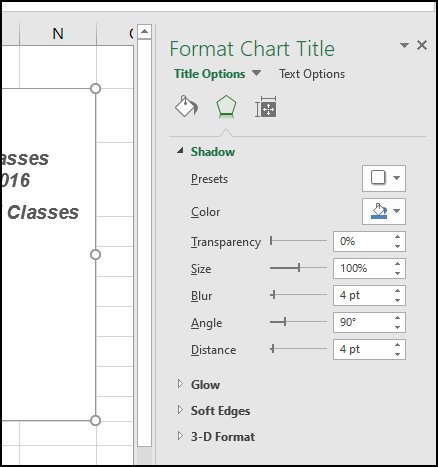
\includegraphics[width=\maxwidth{.95\linewidth}]{gfx/ch04_fig33}
	\caption{Selecting a Title for the Y Axis}
	\label{04:fig33}
\end{figure}

3. Using the Home ribbon, change the font of the axis title to Arial, Bold, size 11.
4. Click in the beginning of the Y axis title and delete the generic title. Type Percent of Enrolled
Excel Students.(see Figure 4.33).


\begin{figure}[H]
	\centering
	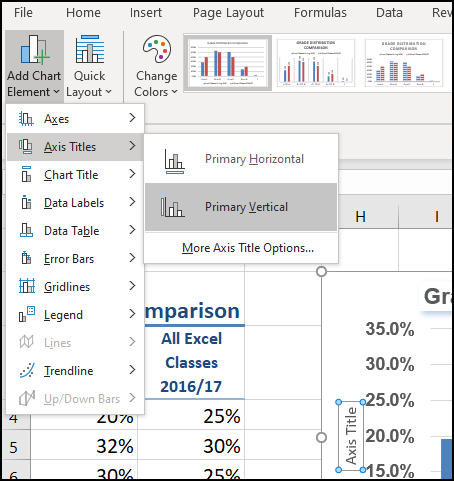
\includegraphics[width=\maxwidth{.95\linewidth}]{gfx/ch04_fig34}
	\caption{Adding and Formatting the Y Axis Title}
	\label{04:fig34}
\end{figure}


Next we will add the title for the X axis.

1. On the Design tab select the Add Chart Element button, then Axis Titles, then Primary
Horizontal.
2. Using the Home ribbon, change the font of the axis title to Arial, Bold, size 11.
3. Click in the beginning of the X axis title and delete the generic title. Type Final Course Grade.
Figure 4.34 shows the added titles for the X and Y axes. The titles provide definitions for the
grade categories along the X axis as well as the percentages on the Y axis.
4. Save your work.

\begin{figure}[H]
	\centering
	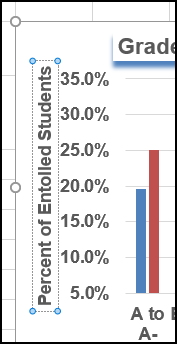
\includegraphics[width=\maxwidth{.95\linewidth}]{gfx/ch04_fig35}
	\caption{X and Y Axis Titles Added}
	\label{04:fig35}
\end{figure}

\begin{center}
	\begin{sklbox}{Skill Refresher}
		\textbf{X and Y Axis Titles}
		\\
		\begin{itemize}
			\setlength{\itemsep}{0pt}
			\setlength{\parskip}{0pt}
			\setlength{\parsep}{0pt}

			\item On the Design tab select the Add Chart Element button.
			\item Click anywhere on the chart to activate it.
			\item Select one of the options from the second drop-down list.
			\item Click in the axis title to remove the generic title and type a new title.
			
		\end{itemize}
	\end{sklbox}
\end{center}

\subsection{Data Series Labels and Formats}

Adding labels to the data series of a chart is a key formatting feature. A data series is the item
that is being displayed graphically on a chart. For example, the blue bars on the Grade Distribution

Comparison chart represent one data series. We can add labels at the end of each bar to show the
exact percentage the bar represents. In addition, we can add other formatting enhancements to the
data series, such as changing the color of the bars or adding an effect. The following steps explain how
to add these labels and formats to the chart:

1. Click on any of the the red bars representing the All Excel Classes data series on the Grade
Distribution Comparison chart in the Grade Distribution worksheet. Clicking one bar
automatically activates all bars in the data series. If you click a bar a second time, only that bar is
activated.
2. Right click and select Format Data Series to open up the Format Data Series pane.
3. Click the Fill and Line (paint bucket) button to bring up the Fill and Border group of
commands.
4. Click the word Fill (if needed) to expand the list of Fill options.
5. Select Pattern Fill. Then select 30% (fifth column, top row). Changing your fill pattern to a
pattern makes it easier to distinguish between the data series when you print or view your chart
in black and white. While you are there, make changes to the fill by experimenting with different
foreground and background colors.
6. Close the Format Data Series pane.



\begin{figure}[H]
	\centering
	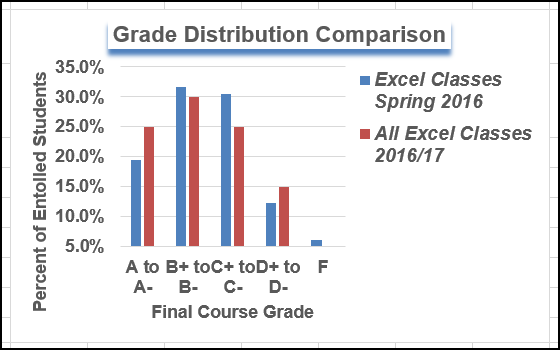
\includegraphics[width=\maxwidth{.95\linewidth}]{gfx/ch04_fig36}
	\caption{Changing the Fill of a Data Series}
	\label{04:fig36}
\end{figure}

Now we are going to add the Data Labels at the end of the columns.

1. Be sure that your entire chart is selected, not just one of the data series. Click the Design tab in
the Chart Tools section of the ribbon.
2. On the Design tab select the Add Chart Element button, then Data Labels, then Outside
End (see Figure 4.36.)
3. Click on one of the Data Labels. Note that all of the data labels for that data series are selected.
4. Using the Home ribbon, change the font to Arial, Bold, size 9.
5. Click on one of the data labels for the other data series. Format those data labels as Arial, Bold,
size 9 as well.
6. Save your work.



\begin{figure}[H]
	\centering
	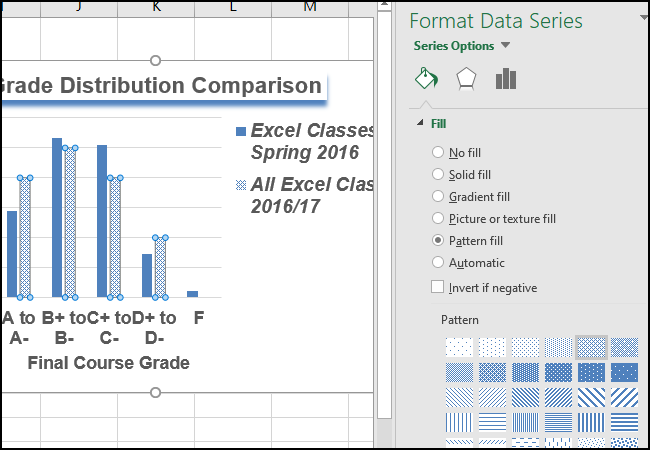
\includegraphics[width=\maxwidth{.95\linewidth}]{gfx/ch04_fig37}
	\caption{Adding Labels to a Data Series}
	\label{04:fig37}
\end{figure}


Figure 4.37 shows the Grade Distribution Comparison chart with the completed formatting
adjustments and labels added to the data series. Note that we can move each individual data label. This
might be necessary if two data labels overlap or if a data label falls in the middle of a grid line. To move
an individual data label, click it twice, then click and drag.



\begin{figure}[H]
	\centering
	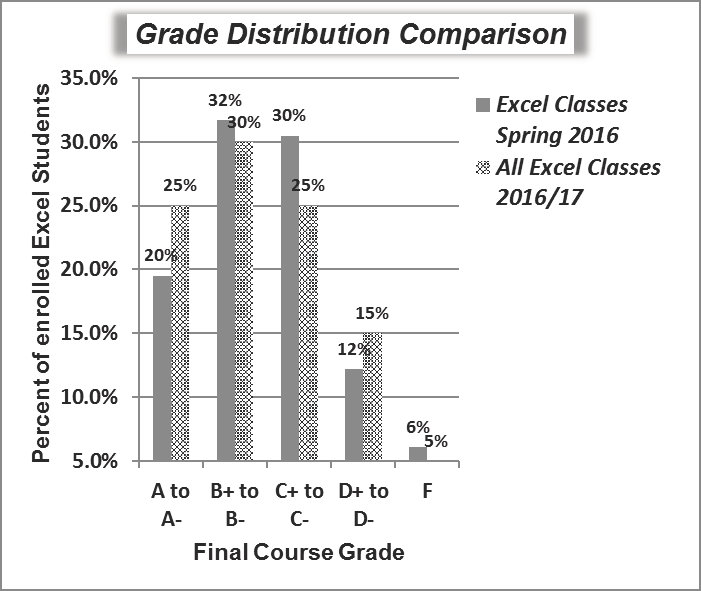
\includegraphics[width=\maxwidth{.95\linewidth}]{gfx/ch04_fig38}
	\caption{Completed Formatting Adjustments for the Data Series}
	\label{04:fig38}
\end{figure}

\begin{center}
	\begin{sklbox}{Skill Refresher}
		\textbf{Adding Data Labels}
		\\
		\begin{itemize}
			\setlength{\itemsep}{0pt}
			\setlength{\parskip}{0pt}
			\setlength{\parsep}{0pt}

			\item Click anywhere on the chart to activate it.
			\item Click the Design tab in the Chart Tools section of the ribbon.
			\item Click the Add Chart Element in the Chart Layout group.
			\item Select Data Labels
			\item Select one of the preset positions from the drop-down list.
			
		\end{itemize}
	\end{sklbox}
\end{center}

\begin{center}
	\begin{sklbox}{Skill Refresher}
		\textbf{Formatting a Data Series}
		\\
		\begin{itemize}
			\setlength{\itemsep}{0pt}
			\setlength{\parskip}{0pt}
			\setlength{\parsep}{0pt}
			
			\item Click any bar or line for a data series.
			\item Right click to activate the Format Data Series pane.
			\item Use the formatting tools in the pane to make changes to the data series.
			
		\end{itemize}
	\end{sklbox}
\end{center}

\subsection{Adding Series Lines and Annotations to a Chart}

The last formatting features we will demonstrate are adding series lines and annotations to a chart.
To demonstrate these skills, we will use the Change in Enrollment Statistics Spend Source stacked
column chart. Series lines are commonly used in stacked column charts to show the change from one
stack to the next. Annotations are useful for clarifying the data presented in a chart or for identifying
data sources. In addition to demonstrating these skills, we will review several of the formatting skills
that were covered in this section. The following steps include the skills review as well as the new
formatting features:

1. Locate the Enrollment by Race stacked column chart on the Enrollment Statistics worksheet.
Activate the chart by clicking anywhere inside the chart perimeter.
2. Move the chart to a separate chart sheet by clicking the Move Chart button in the Design tab of
the ribbon. Type the following in the New sheet input box: Enrollment by Race Chart. Click
the OK button.
3. Click anywhere on the data table (on the x axis) to activate it. Using the Home ribbon, change
the font to Arial, Bold, size 12.
4. Activate the Y axis and apply the same formatting adjustments as stated in step 3.
5. Add a Y axis title using Add Chart Elements – Axis Titles – then More Axis Title Options.
6. In the Format Axis Title pane change the fill color and border to colors of your choice.
7. Then, using the Home tab of the ribbon, change the font to Arial, Bold, size 14.
8. Change the text of the Y axis title to Percent Enrollment by Race.
9. Check the horizontal axis to see if this process created an extra axis title there. If it did, delete it.
10. Activate the title of the chart by clicking it once. The Format Chart Title pane should be open.
If not, right click the Chart title and select Format Chart Title from the menu. Change
the fill and border to match your vertical Axis label.
11. Then, using the Home tab of the ribbon, change the font of the chart title to Arial, Bold, size 20.
12. Close the Formatting pane.
13. Click the Add Chart Elements tool (Design tab), then Lines, then Series Lines.
This adds lines to the chart, connecting each data series between the three stacks (see Figure
4.38).



\begin{figure}[H]
	\centering
	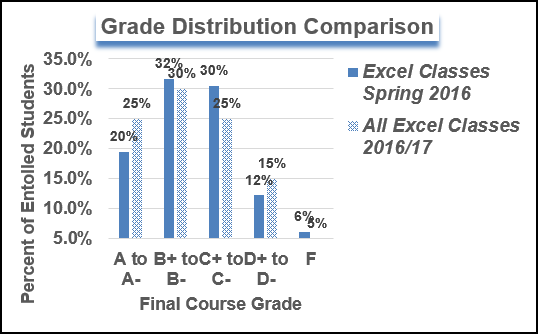
\includegraphics[width=\maxwidth{.95\linewidth}]{gfx/ch04_fig39}
	\caption{Selecting the Series Lines Option}
	\label{04:fig39}
\end{figure}

1. Right click on any of the series lines added to the chart. Clicking one line will activate all lines
on the chart. (If the Format Pane is open, you will not need to right click. Just left click on any of
the series lines to change the format pane to Format Series Lines)
2. Select Format Series Lines. This will open the Format Series Lines pane.
3. Change the width to 2.25.
4. Close the Format Series Lines pane.

Figure 4.39 shows the appearance of the chart with the series lines connecting the two stacks. This
formatting enhancement is common for stacked column charts. The lines help focus the audience’s
attention to changes in the percent of total trend.



\begin{figure}[H]
	\centering
	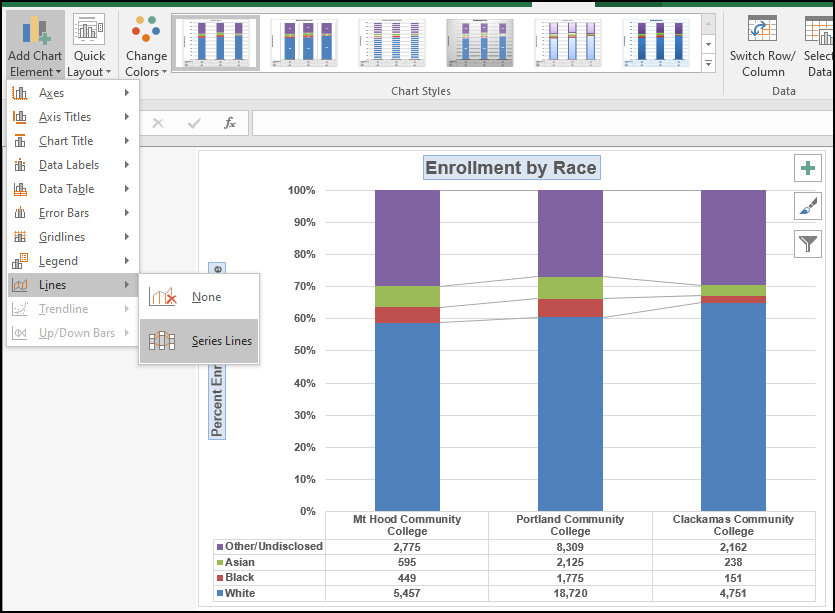
\includegraphics[width=\maxwidth{.95\linewidth}]{gfx/ch04_fig40}
	\caption{Series Lines Added to the Stacked Column Chart}
	\label{04:fig40}
\end{figure}


Our chart demonstrates the percentage differences in enrollment between the community colleges.
But, it would be handy to know the total Enrollment at each of the colleges. To display that, we will
add text boxes above each column. To start with, we need to make room for the text boxes.

1. Select the Plot Area. Place your cursor on the top center handle of the Plot Area and drag down
about ½ inch.


\begin{figure}[H]
	\centering
	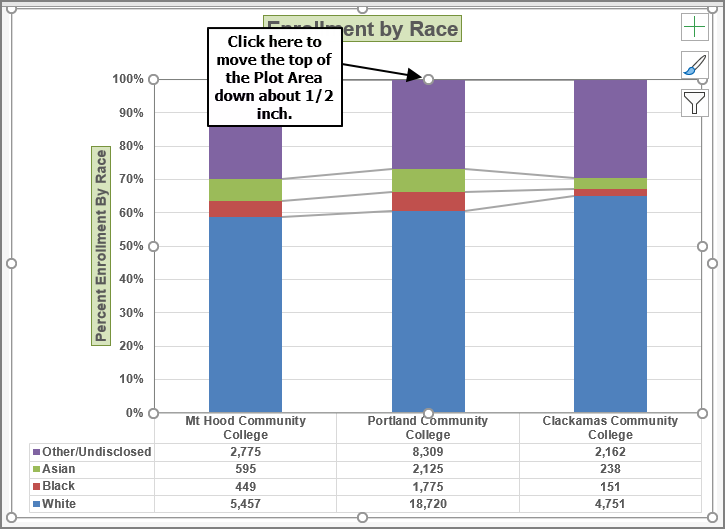
\includegraphics[width=\maxwidth{.95\linewidth}]{gfx/ch04_fig41}
	\caption{Resizing the Plot Area}
	\label{04:fig41}
\end{figure}


\subsection{Add Text Boxes to Include Additional Information in the Chart.}

1. Click the Text Box button in the Text group on the Insert tab of the ribbon (see Figure 4.41).
2. Place the mouse pointer on the left edge of the chart area approximately one-quarter inch from

the top. Click and drag a rectangle approximately one and a half inches wide and one-quarter
inch high (see Figure 4.41). Don’t worry if it’s not exact – you can move and resize text boxes at
any time.
3.   Type Total Enrollment. This tells the audience the size of each school.
4.   Select all of the text in the text box. (You can either highlight the text or click on the border of
the text box once to select all of the text). Using the Home tab of the ribbon, change the font to
Arial, size 14.
5.   Repeat the process to add and format text boxes above each column. You can try to copy and
paste the text boxes if you would like to save time.
6.   In each text box, type the Total Enrollment for each school:

* Mt Hood - 9,276
* Portland - 30,929
* Clackamas - 7,302

7. Save your work.


\begin{figure}[H]
	\centering
	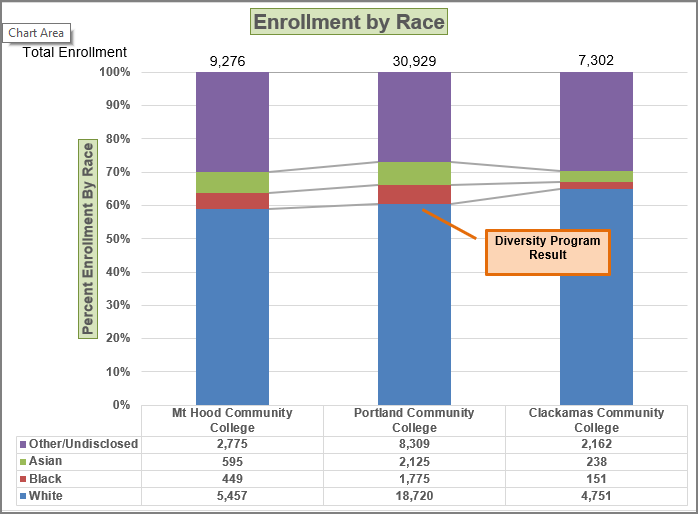
\includegraphics[width=\maxwidth{.95\linewidth}]{gfx/ch04_fig42}
	\caption{Completed Stacked Column Chart}
	\label{04:fig42}
\end{figure}


\begin{center}
	\begin{sklbox}{Skill Refresher}
		\textbf{Adding Series Lines}
		\\
		\begin{itemize}
			\setlength{\itemsep}{0pt}
			\setlength{\parskip}{0pt}
			\setlength{\parsep}{0pt}
			
			\item Click anywhere on the chart area.
			\item Click the Layout tab of the ribbon.
			\item Click the Lines button in the Analysis group of commands.
			\item Click the Series Lines option from the drop-down list.
			
		\end{itemize}
	\end{sklbox}
\end{center}

\begin{center}
	\begin{sklbox}{Skill Refresher}
		\textbf{Adding Annotations}
		\\
		\begin{itemize}
			\setlength{\itemsep}{0pt}
			\setlength{\parskip}{0pt}
			\setlength{\parsep}{0pt}
			
			\item Click anywhere on the chart area.
			\item Click the Insert tab of the ribbon.
			\item Click the Text Box button in the Text group of commands.
			\item Click and drag the size of the text box needed on the chart.
			\item Apply any desired format changes from the Home tab of the ribbon.
			\item Type the desired text.
			
		\end{itemize}
	\end{sklbox}
\end{center}

\begin{center}
	\begin{infobox}{Integrity Check}
		\textbf{Annotations and Axis Titles}
		\\
		\\
		Although adding annotations and axis titles can be a tedious process, doing so maintains a high level of integrity for charts. People can misinterpret the message being conveyed by the chart if they make inaccurate assumptions about the values displayed. Axis titles and annotations help prevent readers from making false assumptions and ensure that readers see the most accurate representation of the message being conveyed by the chart.		
	\end{infobox}
\end{center}


\begin{center}
	\begin{tkwbox}{Key Take-Aways}
		\textbf{Save}
		\\
		\begin{itemize}
			\setlength{\itemsep}{0pt}
			\setlength{\parskip}{0pt}
			\setlength{\parsep}{0pt}

			\item Applying appropriate formatting techniques is critical for making a chart easier to read.
			\item Many formatting commands in the Home tab of the ribbon can be applied to a chart.
			\item To change the number format for a data label, you must use the Number section in the Format Data Labels dialog box. You cannot use the Number format commands in the Home tab of the ribbon.
			\item To change the number format for the values on the Y axis, and the X axis in the case of a scatter chart, you must use the Number section of the Format Axis dialog box. You cannot use the Number format commands
			in the Home tab of the ribbon.
			\item Axis titles and annotations help prevent false assumptions from being made and ensure that the reader sees the most accurate representation of the information presented on a chart.
			
		\end{itemize}
	\end{tkwbox}
\end{center}


\section{Using Charts With Microsoft® Word® and Microsoft® Powerpoint®}


\begin{center}
	\begin{objbox}{Learning Objectives}
		\begin{itemize}
			\setlength{\itemsep}{0pt}
			\setlength{\parskip}{0pt}
			\setlength{\parsep}{0pt}

			\item Learn how to paste an image of an Excel chart into a Word document.
			\item Learn how to paste a link to an Excel chart into a PowerPoint slide.
			
		\end{itemize}
	\end{objbox}
\end{center}

Charts that are created in Excel are commonly used in Microsoft Word documents or for
presentations that use Microsoft PowerPoint slides. Excel provides options for pasting an image of a
chart into either a Word document or a PowerPoint slide. You can also establish a link to your Excel
charts so that if you change the data in your Excel file, it is automatically reflected in your Word or
PowerPoint files. We will demonstrate both methods in this section.

\subsection{Pasting a Chart Image Into Word}

For this exercise you will need two files:

• The Excel spreadsheet you have been working with in this chapter — CH4 Charting.
• A Word document data file — CH4 Diversity

Excel charts can be valuable tools for explaining quantitative data in a written report. Reports that
address business plans, public policies, budgets, and so on all involve quantitative data. For this
example, we will assume that the Change in Enrollment Statistics Spend Source stacked column chart
is being used in a student’s written report (see Figure 4.44). The following steps demonstrate how to
paste an image, or picture, of this chart into a Word document:

1. Open CH4 Diversity. Save it as CH4 Diversity in Enrollment in Community Colleges
2. Click below the figure heading in the Word document that reads: Figure 1: Enrollment by
Race. The image of the stacked column chart will be placed below this heading.
3. If needed, open the Excel file you have been working with (CH4 Charting). Activate the
Enrollment by Race chart in the Enrollment by Race Chart sheet.
4. Click the down arrow on the Copy button in the Home tab of the ribbon. Select Copy as
Picture
5. Select OK — Accepting the Copy Pictures defaults:


* As shown on Screen
* Picture

6. Go back to the CH4 Diversity in Enrollment in Community Colleges Word document by clicking the
file in the taskbar.
7. Confirm that the insertion point is below the Figure 1: Enrollment by Race heading (see Figure
4.42) and click the Paste button in the Home tab of the ribbon ( or press Crtl-V).


\begin{figure}[H]
	\centering
	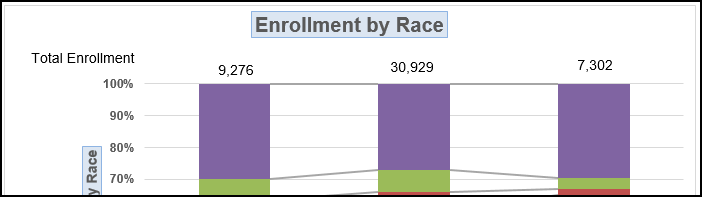
\includegraphics[width=\maxwidth{.95\linewidth}]{gfx/ch04_fig43}
	\caption{Paste Picture in Word}
	\label{04:fig43}
\end{figure}


Oh no!! The picture is so big that it falls on to the next page. We will need to change its size.

1. Click anywhere on the picture of the chart to activate it.
2. Click the Format tab under the Picture Tools section of the ribbon (see Figure 4.43).
3. Click the down arrow on the Shape Width button in the Size group of commands. Continue to
click the down arrow until the width of the picture is 5.4.” As you reduce the width of the
picture, the height is automatically reduced as well. (The height should be about 3.92'')
4. To center the chart on the page, make sure the chart is activated. Then go to the Home tab, to
the Paragraph group, and select Center.
5. Save your work.


\begin{figure}[H]
	\centering
	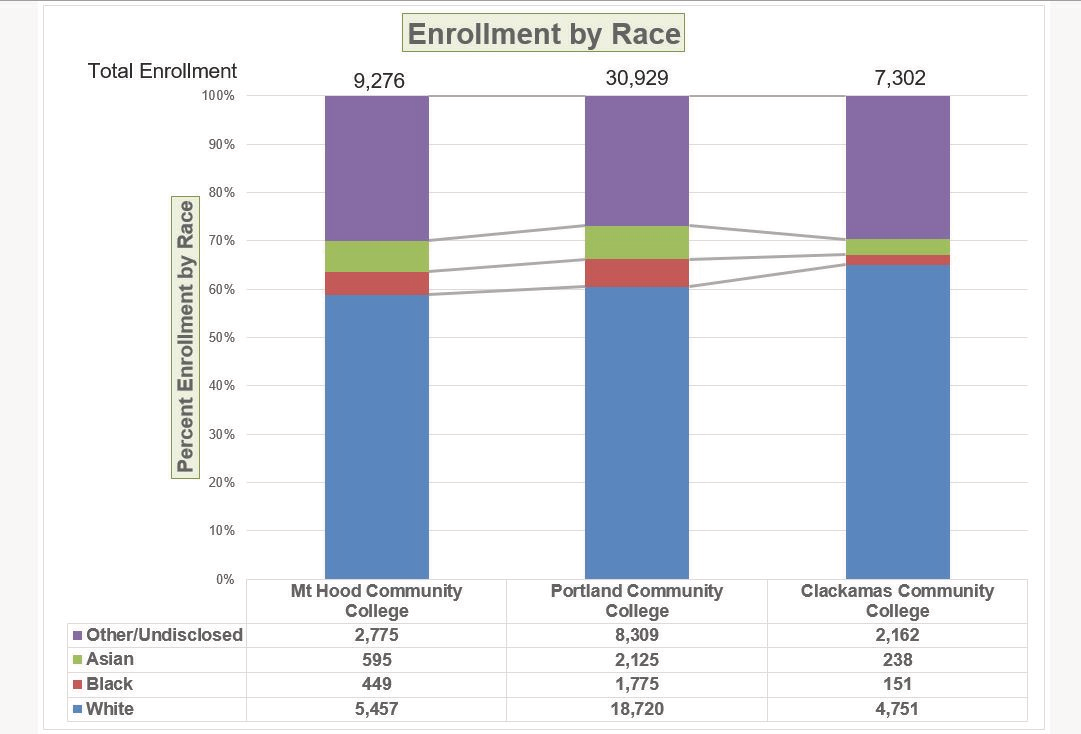
\includegraphics[width=\maxwidth{.95\linewidth}]{gfx/ch04_fig44}
	\caption{Changing the Size of a Picture in Word}
	\label{04:fig44}
\end{figure}


Figure 4.44 shows the final appearance of the Enrollment by Race Source chart pasted into a Word
document. It is best to use either the Shape Width or Shape Height buttons to reduce the size of
the chart. Using either button automatically reduces the height and width of the chart in proper
proportion. If you choose to use the sizing handles to resize the chart, holding the SHIFT key while
clicking and dragging on a corner sizing handle will also keep the chart in proper proportion.


\begin{figure}[H]
	\centering
	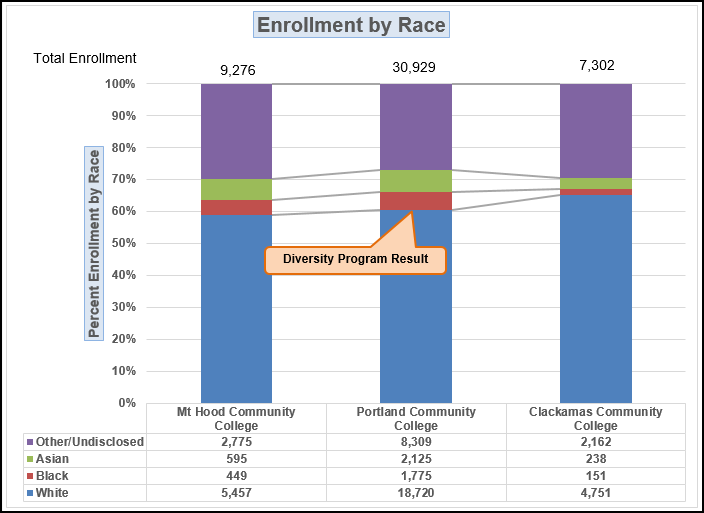
\includegraphics[width=\maxwidth{.95\linewidth}]{gfx/ch04_fig45}
	\caption{Final Appearance of Pasting a Chart Image into Word}
	\label{04:fig45}
\end{figure}

\begin{center}
	\begin{sklbox}{Skill Refresher}
		\textbf{Pasting a Chart Image into Word}
		\\
		\begin{itemize}
			\setlength{\itemsep}{0pt}
			\setlength{\parskip}{0pt}
			\setlength{\parsep}{0pt}

			\item Activate an Excel chart and click the Copy button in the Home tab of the ribbon.
			\item Click on the location in the Word document where the Excel chart will be pasted.
			\item Click the down arrow of the Paste button in the Home tab of the ribbon.
			\item Click the Picture option from the drop-down list.
			\item Click the Format tab in the Picture Tools section of the ribbon.
			\item Resize the picture by clicking the up or down arrow on the Shape Width or Shape Height buttons.
			
		\end{itemize}
	\end{sklbox}
\end{center}

\subsection{Pasting a Linked Chart Image Into Powerpoint}

For this exercise you will need two files:

• The Excel spreadsheet you have been working with in this chapter — CH4 Charting.
• A PowerPoint data file – CH4 Diversity.

Microsoft PowerPoint is perhaps the most commonly used tool for delivering live presentations. The
charts used in a live presentation are critical for efficiently delivering your ideas to an audience.
Similar to written documents, a wide range of presentations may require the explanation of
quantitative data. This demonstration includes a PowerPoint slide that could be used in a
presentation. We will paste the Enrollment by Race chart into this PowerPoint slide. However, instead
of pasting an image, as demonstrated in the Word document, we will establish a link to the Excel file.
As a result, if we change the chart in the Excel file, the change will be reflected in the PowerPoint file.
The following steps explain how to accomplish this:

1. Open CH4 Diversity.pptx. Save it as CH4 Diversity in Enrollment in Community Colleges.
2. Navigate to Slide 6 – Diversity in Enrollment. This is the slide where you will place the linked
chart.
3. If needed, open the Excel file you have been working with (CH4 Charting). Activate the
Enrollment by Race chart in the Enrollment by Race Chart sheet.
4. Click the down arrow on the Copy button in the Home tab of the ribbon. Select Copy (not
Copy as Picture.)
5. Go back to the CH4 Diversity in Enrollment in Community Colleges presenation by clicking the file
in the taskbar.
6. Make sure you are still on Slide 6 – Diversity in Enrollment. Click on the outside edge of the
empty prompt box on the right.
7. Click the down arrow below the Paste button in the Home tab of the ribbon in the PowerPoint
file.
8. Hover over each of the Paste Options until you find Keep Source Formatting \& Link Data (see
Figure 4.45). Select this option. This pastes an image of the Excel chart into the PowerPoint
slide. In addition, a link is created so that any changes made to the chart (in Excel) appear on the
PowerPoint slide.



\begin{figure}[H]
	\centering
	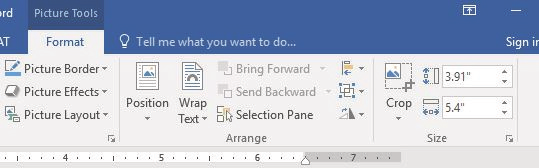
\includegraphics[width=\maxwidth{.95\linewidth}]{gfx/ch04_fig46}
	\caption{Creating a Link to an Excel Chart in PowerPoint}
	\label{04:fig46}
\end{figure}


Next we need to make some changes to clean up the chart a bit. First, we are going to apply a different
chart style.

1. Click anywhere in the plot area of the column chart pasted into the PowerPoint slide. You will
see the same Excel Chart Tools tabs added to the ribbon (see Figure 4.46).
2. On the Design tab, select Style 8 in the Chart Style group.


\begin{figure}[H]
	\centering
	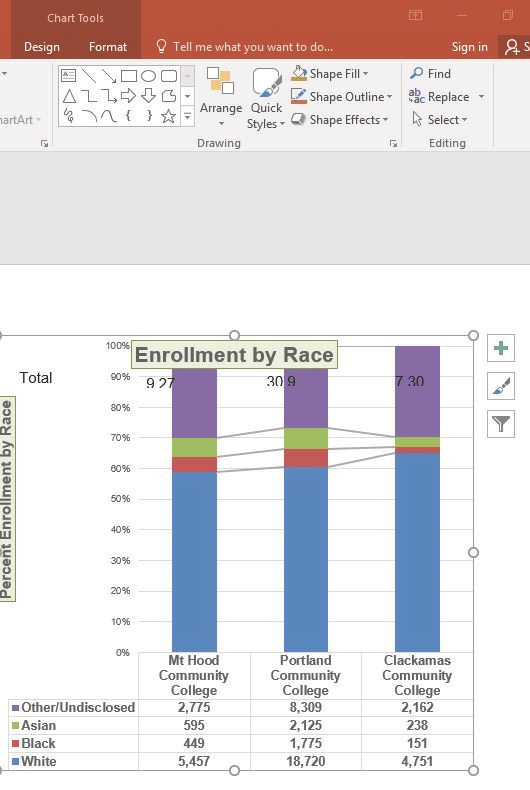
\includegraphics[width=\maxwidth{.95\linewidth}]{gfx/ch04_fig47}
	\caption{Modifying an Excel Chart Pasted into a PowerPoint Slide}
	\label{04:fig47}
\end{figure}

Paste linking this chart caused trouble with the text boxes we added, so next we are going to delete
them.

1. Select each text box by clicking on the outside edge of the text box with the four-headed arrow.

Press the delete key on your keyboard. Be sure that the insertion point is NOT blinking inside
the text box. If it is, you will be editing the contents of the text box instead of deleting the actual
text box.

The benefit of adding this chart to the presentation as a link is that it will automatically update when
you change the data in the linked spreadsheet file.

1. Return to your CH4 Charting Excel file.
2. Select the Enrollment Statistics worksheet (the one with the Enrollment data.) Change the
value in cell D3 to 1000. You have just changed the number of white students at Clackamas
Community College to 1000. This isn’t true, but you want to change the data enough to see the
effect in the charts.
3. Select the Enrollment by Race Chart worksheet. Notice how the chart has changed.
4. Return to the Diversity in Enrollment in Community Colleges PowerPoint file by clicking the
file in the taskbar.
5. On Slide6, you should see the updated chart (see Figure 4.47).
6. If the chart has not changed; be sure that your chart is selected, click the Design tab in the Chart
Tools section of the ribbon. Click the Refresh Data button. The change made in the Excel
workbook is now reflected on the PowerPoint slide.
7. If that still doesn’t work, you may have created a “normal” link — instead of a Paste Link.
Delete the chart and follow the steps again. Start from the beginning of this section.
8. Save your work. You will submit both the Word and PowerPoint files, along with the Excel file,
at the end of the next section.

Figure 4.47 shows the appearance of the column chart after the change was made in the Enrollment
Statistics worksheet in the Excel file. Note that the Data Chart at the bottom reflects the new number,
too. The change that was made in the Excel file will appear in the PowerPoint file after clicking the
Refresh Data button.



\begin{figure}[H]
	\centering
	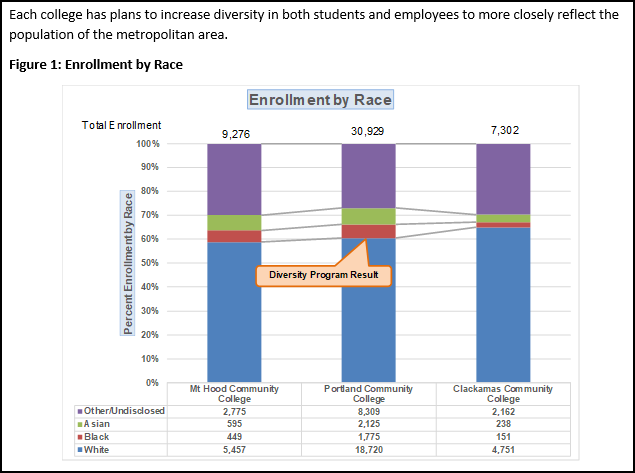
\includegraphics[width=\maxwidth{.95\linewidth}]{gfx/ch04_fig48}
	\caption{Styled and Updated Chart}
	\label{04:fig48}
\end{figure}

\begin{center}
	\begin{sklbox}{Skill Refresher}
		\textbf{Pasting a Linked Chart Image into PowerPoint}
		\\
		\begin{itemize}
			\setlength{\itemsep}{0pt}
			\setlength{\parskip}{0pt}
			\setlength{\parsep}{0pt}
			
			\item Activate an Excel chart and click the Copy button in the Home tab of the ribbon.
			\item Click in the PowerPoint slide where the Excel chart will be pasted.
			\item Click the down arrow of the Paste button in the Home tab of the ribbon.
			\item Click the Keep Source Formatting \& Link Data option from the drop-down list.
			\item Click the Refresh Data button in the Design tab of the ribbon to ensure any changes in the Excel file are reflected in the chart.
			
		\end{itemize}
	\end{sklbox}
\end{center}

\begin{center}
	\begin{infobox}{Integrity Check}
		\textbf{Refreshing Linked Charts in PowerPoint and Word}
		\\
		\\
		When creating a link to a chart in Word or PowerPoint, the data must be refreshed when there are changes in the Excel workbook. This is especially true if the changes are made in the Excel file prior to opening the Word or PowerPoint file that contains a link to a chart. To refresh the chart, make sure it is activated, then click the Refresh Data button in the Design tab of the ribbon. Forgetting this step can result in old or erroneous data being displayed on the chart.
	\end{infobox}
\end{center}



\begin{center}
	\begin{tkwbox}{Key Take-Aways}
		\textbf{Save}
		\\
		\begin{itemize}
			\setlength{\itemsep}{0pt}
			\setlength{\parskip}{0pt}
			\setlength{\parsep}{0pt}

			\item When pasting an image of an Excel chart into a Word document or PowerPoint file, use the Picture option from the Paste drop-down list of options if you want the image to act as an image. You will not be able to make any changes to the content of the picture.
			\item When creating a link to a chart in Word or PowerPoint, you may need to refresh the data if you make any changes in the originating spreadsheet. You should not use the Picture option.
					
		\end{itemize}
	\end{tkwbox}
\end{center}

\begin{center}
	\begin{infobox}{Integrity Check}
		\textbf{Severed Link?}
		\\
		\\
		When creating a link to an Excel chart in Word or PowerPoint, the Excel workbook must stay in its original location on the computer or network. If the workbook is moved or deleted, an error message will be generated when the link in your Word or PowerPoint file is updated. An error is also generated if the Excel workbook is saved on a network drive that the computer cannot access. These errors occur because the link to the Excel workbook has been severed. Therefore, if a USB drive is being used for a presentation then all of the linked Excel workbooks must be moved to the USB drive before establishing the Word or PowerPoint link.
	\end{infobox}
\end{center}


\section{Preparing to Print}


\begin{center}
	\begin{objbox}{Learning Objectives}
		\begin{itemize}
			\setlength{\itemsep}{0pt}
			\setlength{\parskip}{0pt}
			\setlength{\parsep}{0pt}

			\item Review each worksheet in a workbook in Print Preview.
			\item Modify worksheets as needed to professionally print data and charts.
			
		\end{itemize}
	\end{objbox}
\end{center}


In this section we will take a look at each of the worksheets created in the previous sections. Since
these worksheets contain a combination of data and charts, there are specific things to watch for if
you will be printing the sheets.

We will start by looking at each worksheet in Print Preview in Backstage View. We will then make
any changes necessary, such as changing the orientation and scaling, or moving charts around on the
worksheet. To make sure we don’t miss any worksheets, we are going to review the worksheets in the
order they appear in the tabs.

\subsection{Previewing Chart Sheets for Printing}

Data file: Continue with CH4 Charting.

The first worksheet, Closing Prices, is a chart sheet. This means that it does not contain any data;
remember that chart sheets just contain charts. We still need to review it in Print Preview.

1.   Click on the Closing Prices worksheet tab.
2.   Go to Print Preview by clicking Print in Backstage View.
3.   Notice that the chart will print on the entire page, in Landscape orientation.
4.   There is nothing to change. Exit Backstage View.

PRINTING WORKSHEETS WITH DATA AND CHARTS

The next worksheet (Stock Trend) has a lot of data and multiple charts. We need to print the data and
the charts, which will require some modifications of the page setup.

1.   Click on the Stock Trend worksheet tab.
2.   Go to Print Preview by clicking Print in Backstage View.
3.   Notice that this worksheet is currently printing on seven pages.
4.   As you click through each page you should make the following observations:


* The data is split between the first and third pages.
* The line chart starts on the first page, but part of it is also on the second page.
* The double-line chart starts on the third page, and then finishes on the fifth page.
* The fourth and sixth pages are blank.
* The last page has a column of seemingly random numbers.

5. Exit Backstage View.

The first thing we are going to do is remove the numbers that are appearing on page 7. To do this,
we will hide the column where they are being stored. We are going to hide the column, instead of
deleting the numbers, in case the numbers are being utilized somewhere else in the workbook.

1. Scroll to the right on the worksheet until you find the numbers in column AH.
2. Click anywhere in column AH.
3. On the Home ribbon, click the Format button in the Cells group.
4. In the Visibility section, select Hide \& Unhide then select Hide Columns (see Figure 4.64).
5. The visible column headings should now go from AG to AI.
6. Return to Print Preview in Backstage View to see the changes to the printed worksheet.
7. Notice that there are now five pages. The data and charts are still splitting across multiple
pages, but the numbers in column AH are no longer going to print.
8. Remain in Backstage View for the next steps.


\begin{figure}[H]
	\centering
	\includegraphics[width=\maxwidth{.95\linewidth}]{gfx/ch04_fig49}
	\caption{Hide Columns in Format Menu}
	\label{04:fig49}
\end{figure}

The data is still split between pages 2 and 3, and the charts are splitting oddly as well. The first step
we will try to fix these issues is to change the page orientation and scaling.

1. While still in Backstage View, change the page orientation to Landscape (use the Orientation
drop-down menu in the Settings section).
2. This puts all of the data on one sheet, but the charts are still split between multiple pages.


3. Change the page scaling to Fit Sheet on One Page (use the Scaling drop-down menu in the
Settings section).
4. This fits everything on one page, but it is too small to be able to read.
5. Change the page scaling back to No Scaling.

The next thing we will try is moving one, or both, of the charts. In order to move the charts, we need
to exit out of Backstage View.

1. Exit Backstage View.
2. Switch to the View ribbon and then select Page Break Preview. Your screen should look similar
to Figure 4.65. (Remember that the dotted blue lines indicate automatic page breaks.)
3. Move the 24 Month Comparison (double-line) chart closer to the top of its page.
4. Move the May 2014-2015 Trend for NASDAQ Sales Volume (line chart) so that it is under the
24 Month Comparison chart.
5. The link to the data source is still at the bottom of page 2 (in A50:A51) so you need to move it as
well. Using your preferred method, move the text from A50:A51 to M31:M32.
6. Now your screen should look similar to Figure 4.66.


\begin{figure}[H]
	\centering
	\includegraphics[width=\maxwidth{.95\linewidth}]{gfx/ch04_fig50}
	\caption{Page Break Preview before moving the charts in Step 3}
	\label{04:fig50}
\end{figure}

\begin{figure}[H]
	\centering
	\includegraphics[width=\maxwidth{.95\linewidth}]{gfx/ch04_fig51}
	\caption{Page Break Preview after moving the charts and text}
	\label{04:fig51}
\end{figure}




We don’t want the data source link text to print on its own page, but there is no room to move it onto
the same page as the charts. To fix this, we are going to remove the automatic page break between the
charts and the text in M31:M32.

1. Place your pointer on the horizontal blue dashed line (automatic page break) between the line
chart and the Data Source link text.
2. When your pointer changes to the double arrow (pointing up and down), drag the page break
down into the gray area. This removes the page break.
3. If your vertical automatic page break between columns L and M moves, drag it back between
columns L and M. This will make it a solid blue line, which will no longer adjust automatically.
4. Your screen should now look like Figure 4.67.



\begin{figure}[H]
	\centering
	\includegraphics[width=\maxwidth{.95\linewidth}]{gfx/ch04_fig52}
	\caption{Page Break Preview after removing a page break}
	\label{04:fig52}
\end{figure}

Now you need to do one final check of this worksheet in Print Preview.

1. Go to Print Preview and look at both pages. Page 1 should contain just the data and page 2
should have both charts and the Data Source link text.
2. Exit Backstage View and save the file.

\subsection{Preview Remaining Worksheets for Printing}

There are four remaining worksheets to be reviewed. Some of them will need minor changes and
some will not need any changes. You will need to preview each one and then make the specified
changes. In the following steps you will preview and modify the next three worksheets.

1. All Excel Classes – this is a chart sheet, so it should not need any changes.
2. Grade Distribution – the chart is split across two pages. Fix this by changing the orientation
(Landscape) and scaling (Fit Sheet on One Page).
3. Enrollment by Race Chart – this is a chart sheet, so it should not need any changes.

\subsection{Printing a Chart Only}

Sometimes you might have a worksheet that has data and a chart, but you only want the chart to print.
That is the case with the Enrollment Statistics worksheet.

1. Switch to the Enrollment Statistics worksheet.
2. Select the chart.
3. Go to Print Preview. Only the chart is printing. (If it shows the data printing along with the chart,
exit Backstage View and be sure to select just the chart on the worksheet.)
4. If needed, change the orientation to Landscape. This orientation looks better when printing just
a chart.

5. Exit Backstage View.

\subsection{Hiding a Worksheet}

You have actually decided that you do not want the Enrollment by Race Chart sheet to be visible at
all, but you do not want to delete it. We are going to hide it from anyone looking at the workbook.

1. Right-click on the Enrollment by Race Chart tab.
2. Select Hide from the menu that appears. The Enrollment by Race Chart sheet should no longer
be visible.
3. Now you want to bring the worksheet back. To unhide it, right-click on any other worksheet
tab and select Unhide from the menu. A list of hidden worksheets will be displayed. Select the
Enrollment by Race Chart and click OK.
4. Save the CH4 Charting workbook.
5. Compare your work (on all of the worksheets) with the self-check answer key (found in the
Course Files link).
6. Submit all three files from this chapter (CH4 Charting.xlsx, CH4 Diversity in Enrollment in
Community Colleges.docx, and CH4 Diversity in Enrollment in Community
Colleges.pptx) as directed by your instructor.





\section{Chapter Practice}




To assess your understanding of the material covered in the chapter, please complete the following
assignments.

Although Excel is primarily used in business and scientific applications, you will find it useful in other
areas of study as well. In these exercises we will use Excel to create charts using historical, health, and
social justice data.

\subsection{Charting Historical Data (Comprehensive Review)}

Download Data File: PR4 Data

Excel is an excellent tool for helping to display historical date. In this exercise we will be examining
ways to display information on minimum mage data and life expectancy.



\subsubsection{Task1 – National Minimum Wage in the Us – 1960-2014}

Since the beginning of the previous century, the United States has set a minimum wage, in order to set
a “floor” beneath which wages cannot fall. Most states have set their own minimum wages, but none
are lower than the national minimum wage. To learn more about the national minimum wage, look
here: \url{https://en.wikipedia.org/wiki/Minimum_wage_in_the_United_States}

1. Open the file named PR4 Data and then Save As PR4 Historical Data.
2. On the Minimum Wage worksheet, select the range B4:C60
3. Select the Insert tab, then the Recommended Chart tool in the Charts group.
Recommended Charts allows users to first see how selected data would be represented on a
variety of chart types before committing to a particular type of chart. Being able to see your data
as it would look in a variety of charts helps you select the kind of chart that best matches your
date.
It does a particularly good job when you want to use dates or years as labels. Sometimes, Excel
gets confused and thinks that dates are part of the data – instead of labels.
4. Select the first Line chart. Press OK.
5. Your line chart is embedded in the Minimum Wage worksheet.
6. Make sure that the upper left corner of your chart is in the upper left corner of E4. The lower
right corner is in the lower right corner of M20.
7. Adjusting the chart title: Click the chart title once. Then click in front of the first letter. You
should see a blinking cursor in front of the letter. This allows you to modify the title of the chart.

8. Type the following in front of the first letter in the chart title: US National
9. While your chart is still selected, select the Design tab. You will find the Chart Styles group in
the middle of the ribbon. If necessary, press the More button to see the available styles.
10. Float your cursor over the available styles so you can see how they will affect your chart. Select
Style 4.
11. The years across the X (category) axis are a little hard to read.
Select the labels. When you have them selected, you will see a box surrounding the list of years.
On the Home tab, in the Alignment Group, select the Orientation tool. Select Angle Counter
Clockwise.
12. Prepare the Minimum Wage worksheet for printing by changing the scaling to Fit Sheet on
One Page.

\subsubsection{Task2 – Oregon: Projected Life Expectancy at Birth}

In the past 40 years, between 1970 and 2010, life expectancy for Oregon men improved by 8.7 years
and for women by 5.5 years. Oregon’s life expectancy has remained slightly higher than the U.S.
average. The life expectancy will continue to improve for both men and women. However, the gain
for men has been outpacing the gain for women. Consequently, the difference between men’s and
women’s life expectancies has continued to shrink.

\url{https://www.oregon.gov/das/OEA/Documents/OR_pop_trend2012.pdf}

1. On the Life Expectancy sheet, select A5:B11
2. Press F11
3. This creates a column chart, and puts it on a separate sheet.
4. Double click the chart sheet tab, change the name to Men.
5. Take a good look at this chart. It is not what we were expecting. Excel has made a mistake and
charted the Birth Year information as though it was data, instead of using it to label the bottom
(category) axis. That needs to be fixed. We need to tell Excel that the data in Column A are labels,
not values.
6. With the chart selected, go to the Design tab, and select the Select Data tool.
This opens the Select Data Source dialog box. The box at the top tells us the range we selected,
which looks fine.

The Legend Entries need to be corrected to fix the issue with the data series (columns). Also, the
Horizontal Axis Labels are just a series of default numbers. They need to be the range that contains
the years.

7. In the Legend Entries, click in the small box in front of Birth Year to remove the check mark.
This will remove the Birth Year as a data series on the chart.
8. In the Horizontal (Category) Axis Labels box, press the Edit button. This will open the Axis
Labels dialog box. Press the Select range button.
9. Navigate to the Life Expectancy tab and select A6:A11. After “=’Life Expectancy’!$A$6:$A$11”
is displayed in the box, press the Select Range button. Press OK.
Press OK
10. Change the chart title so that it reads: Life Expectancy for Oregon Men.


11. Remove the Legend from the bottom of the chart by right-clicking on it and selecting Delete.
12. Return to the Life Expectancy tab, select A5:All , C5:C11 (Select the first range, hold down the
CTRL key, select the next to select both noncontiguous ranges at the same time.
13. Repeat steps 2-11 above to create a matching chart for Life Expectancy for Oregon Women.
14. Return to the Life Expectancy tab, select A5:D11
15. Use the Recommended Charts tool to create a simple line chart.
16. Change the Chart Title to Oregon: Projected Life Expectancy at Birth.
17. The green line across the bottom of the chart represents the difference between men’s and
women’s life expectancy. It is not very helpful as it is.
Right click on the green line to open the pop up menu. Select Format Data Series. In the
Format Data Series pane, under the Series Options tab, select the radio button in front of
Secondary Axis.
18. Close the Format Data Series pane.
19. Add a text box that explains the Difference calculation. While the chart is still selected:

1.   On the Insert tab, on the right side of the ribbon, find Text. Select the Text Box tool.
2.   When you select it, your cursor will turn into cross hair (thin black plus sign)
3.   Click once in the lower left corner of your chart. This creates a text box.
4.   Type the following into the text box: Difference = Female life expectancy minus male.
Move or resize the text box if you wish.

20.   Move or resize your chart so that it no longer is on top of the spreadsheet data.
21.   Use the Chart Styles tools to change your chart to something a bit more dramatic.
22.   Preview the Life Expectancy worksheet in Print Preview and make any necessary changes.
23.   Save the PR4 Historical Data workbook.
24.   Compare your work with the self-check answer key (found in the Course Files link) and then
submit the PR4 Historical Data workbook as directed by your instructor.

\section{Scored Assessment}




\subsection{Charting Social Justice Data (Comprehensive Review)}

Download Data File: SC4 Data

\subsubsection{Task 1 International Incarceration Rates}

1. Open the file named SC4 Data and then Save As SC4 Social Justice.
2. On the International tab, use a function in cell D20 to find the average of the Individuals
incarcerated data.
3. Create a bar chart that looks like this:



\begin{figure}[H]
	\centering
	\includegraphics[width=\maxwidth{.95\linewidth}]{gfx/ch04_fig53}
	\caption{International Incarceration Rates}
	\label{04:fig53}
\end{figure}



1. Move and or resize it so that it does not cover any of the data.



2. In cell A25 write a brief note explaining why a bar (or column) chart is a better choice for this
data than a pie chart.
3. Set the Print Area so that everything prints, except for the explanation you added in cell A25.
4. Preview the International worksheet in Print Preview and make any changes needed to print
professionally on one page.

\subsubsection{Task 2 Disenfranchisement Rate}

Felony disenfranchisement is the exclusion from voting of people otherwise eligible to vote (known
as disfranchisement) due to conviction of a criminal offense, usually restricted to the more serious
class of crimes: felonies. Jurisdictions vary as to whether they make such disfranchisement permanent,
or restore suffrage after a person has served a sentence, or completed parole or probation. Affected
individuals suffer “collateral consequences” including loss of access to jobs, housing, and other
facilities.

Opponents have argued that such disfranchisement restricts and conflicts with principles of universal
suffrage. It can affect civic and communal participation in general.

\url{https://en.wikipedia.org/wiki/Felony_disenfranchisement}

On the Disenfranchisement rate sheet, use the Recommended Chart tool to create the following three
charts. Put each chart on its own individual sheet. (Note: Not an object in a spreadsheet.)

Chart1 — Felony Disenfranchisement Rate Washington


\begin{figure}[H]
	\centering
	\includegraphics[width=\maxwidth{.95\linewidth}]{gfx/ch04_fig54}
	\caption{Felony Disenfranchisement Rate Washington}
	\label{04:fig54}
\end{figure}






Chart2 — Felony Disenfranchisement Rate Oregon

\begin{figure}[H]
	\centering
	\includegraphics[width=\maxwidth{.95\linewidth}]{gfx/ch04_fig55}
	\caption{Felony Disenfranchisement Rate Oregon}
	\label{04:fig55}
\end{figure}



Chart3 – Comparison – Oregon and Washington

\begin{figure}[H]
	\centering
	\includegraphics[width=\maxwidth{.95\linewidth}]{gfx/ch04_fig56}
	\caption{Comparison of Oregon and Washington}
	\label{04:fig56}
\end{figure}



Notes

This is called a Clustered column chart in the Recommended charts tool, but it is really a combo chart – with some
data displayed as columns and some data displayed as a line.

You will need to edit the Chart Title.

You may need to adjust the chart size to make it look like the illustration.

Put the chart on its own individual sheet — don’t leave it as an object on the spreadsheet.





Notes:
Take a look at both the Washington and Oregon charts. They are the same kind of chart, but your charts may look
different because the data is a bit different.

To make them more similar – make sure that the vertical axes are the same in both charts. Format the left vertical
(value) axis, so that the Maximum is 20000. Format the right vertical axis, so that the Maximum is .20.




Notes:

Be sure that you have years as labels on the horizontal axis (not 1, 2, 3 . . . )

This chart is on its own separate sheet.




1. When you have completed all three charts, save your work. Preview the worksheet(s) in Print
Preview and make any necessary changes for professional printing.
2. Submit the SC4 Social Justice workbook as directed by your instructor.


